%% We use the memoir class because it offers a many easy to use features.
\documentclass[10pt,a4paper,titlepage, openany]{memoir} %openright, twosided, slides

%% Packages
%% ========

%% LaTeX Font encoding -- DO NOT CHANGE
\usepackage[OT1]{fontenc}

%% Babel provides support for languages.  'english' uses British
%% English hyphenation and text snippets like "Figure" and
%% "Theorem". Use the option 'ngerman' if your document is in German.
%% Use 'american' for American English.  Note that if you change this,
%% the next LaTeX run may show spurious errors.  Simply run it again.
%% If they persist, remove the .aux file and try again.
\usepackage[english]{babel}

%% Input encoding 'utf8'. In some cases you might need 'utf8x' for
%% extra symbols. Not all editors, especially on Windows, are UTF-8
%% capable, so you may want to use 'latin1' instead.
\usepackage[utf8]{inputenc}

%% This changes default fonts for both text and math mode to use Herman Zapfs
%% excellent Palatino font.  Do not change this.
\usepackage[sc]{mathpazo}

%% The AMS-LaTeX extensions for mathematical typesetting.  Do not
%% remove.
\usepackage[intlimits]{amsmath}
\usepackage{amssymb,amsfonts,mathrsfs}

%% NTheorem is a reimplementation of the AMS Theorem package. This
%% will allow us to typeset theorems like examples, proofs and
%% similar.  Do not remove.
%% NOTE: Must be loaded AFTER amsmath, or the \qed placement will
%% break
\usepackage[amsmath,thmmarks]{ntheorem}

%% LaTeX' own graphics handling
\usepackage{graphicx}


%% This allows you to add .pdf files. It is used to add the
%% declaration of originality.
\usepackage{pdfpages}

%% Some more packages that you may want to use.  Have a look at the
%% file, and consult the package docs for each.
%%Custom
\usepackage{enumitem} 	%Anpassbare Enumerates/Itemizes
%%%\usepackage{appendix}	%self-explaining
%% See the TeXed file for more explanations
\usepackage{subcaption} %Multiple figures, 1 caption

%% [OPT] Multi-rowed cells in tabulars
%\usepackage{multirow}


%% [REC] Intelligent cross reference package. This allows for nice
%% combined references that include the reference and a hint to where
%% to look for it.
\usepackage{varioref}

%% [OPT] Easily changeable quotes with \enquote{Text}
%\usepackage[german=swiss]{csquotes}

%% [REC] Format dates and time depending on locale
\usepackage{datetime}

%% [OPT] Provides a \cancel{} command to stroke through mathematics.
%\usepackage{cancel}

%% [NEED] This allows for additional typesetting tools in mathmode.
%% See its excellent documentation.
\usepackage{mathtools}

%% [ADV] Conditional commands
%\usepackage{ifthen}

%% [OPT] Manual large braces or other delimiters.
%\usepackage{bigdelim, bigstrut}

%% [REC] Alternate vector arrows. Use the command \vv{} to get scaled
%% vector arrows.
\usepackage[h]{esvect}

%% [NEED] Some extensions to tabulars and array environments.
\usepackage{array}

%% [OPT] Postscript support via pstricks graphics package. Very
%% diverse applications.
%\usepackage{pstricks,pst-all}

%% [?] This seems to allow us to define some additional counters.
%\usepackage{etex}

%% [ADV] XY-Pic to typeset some matrix-style graphics
%\usepackage[all]{xy}

%% [OPT] This is needed to generate an index at the end of the
%% document.
%\usepackage{makeidx}

%% [OPT] Fancy package for source code listings.  The template text
%% needs it for some LaTeX snippets; remove/adapt the \lstset when you
%% remove the template content.
\usepackage{listings}
\lstset{language=TeX,basicstyle={\normalfont\ttfamily}}

%% [REC] Fancy character protrusion.  Must be loaded after all fonts.
%\usepackage[activate]{pdfcprot}

%% [REC] Nicer tables.  Read the excellent documentation.
\usepackage{booktabs}


%% Our layout configuration.  DO NOT CHANGE.
%% Memoir layout setup

%% NOTE: You are strongly advised not to change any of them unless you
%% know what you are doing.  These settings strongly interact in the
%% final look of the document.

% Dependencies
\usepackage{ETHlogo}

% Turn extra space before chapter headings off.
\setlength{\beforechapskip}{0pt}

\nonzeroparskip
\parindent=0pt
\defaultlists

% Chapter style redefinition
\makeatletter

\if@twoside
  \pagestyle{Ruled}
  \copypagestyle{chapter}{Ruled}
\else
  \pagestyle{ruled}
  \copypagestyle{chapter}{ruled}
\fi
\makeoddhead{chapter}{}{}{}
\makeevenhead{chapter}{}{}{}
\makeheadrule{chapter}{\textwidth}{0pt}
\copypagestyle{abstract}{empty}

\makechapterstyle{bianchimod}{%
  \chapterstyle{default}
  \renewcommand*{\chapnamefont}{\normalfont\Large\sffamily}
  \renewcommand*{\chapnumfont}{\normalfont\Large\sffamily}
  \renewcommand*{\printchaptername}{%
    \chapnamefont\centering\@chapapp}
  \renewcommand*{\printchapternum}{\chapnumfont {\thechapter}}
  \renewcommand*{\chaptitlefont}{\normalfont\huge\sffamily}
  \renewcommand*{\printchaptertitle}[1]{%
    \hrule\vskip\onelineskip \centering \chaptitlefont\textbf{\vphantom{gyM}##1}\par}
  \renewcommand*{\afterchaptertitle}{\vskip\onelineskip \hrule\vskip
    \afterchapskip}
  \renewcommand*{\printchapternonum}{%
    \vphantom{\chapnumfont {9}}\afterchapternum}}

% Use the newly defined style
\chapterstyle{bianchimod}

\setsecheadstyle{\Large\bfseries\sffamily}
\setsubsecheadstyle{\large\bfseries\sffamily}
\setsubsubsecheadstyle{\bfseries\sffamily}
\setparaheadstyle{\normalsize\bfseries\sffamily}
\setsubparaheadstyle{\normalsize\itshape\sffamily}
\setsubparaindent{0pt}

% Set captions to a more separated style for clearness
\captionnamefont{\sffamily\bfseries\footnotesize}
\captiontitlefont{\sffamily\footnotesize}
\setlength{\intextsep}{16pt}
\setlength{\belowcaptionskip}{1pt}

% Set section and TOC numbering depth to subsection
\setsecnumdepth{subsection}
\settocdepth{subsection}

%% Titlepage adjustments
\pretitle{\vspace{0pt plus 0.7fill}\begin{center}\HUGE\sffamily\bfseries}
\posttitle{\end{center}\par}
\preauthor{\par\begin{center}\let\and\\\Large\sffamily}
\postauthor{\end{center}}
\predate{\par\begin{center}\Large\sffamily}
\postdate{\end{center}}

\def\@advisors{}
\newcommand{\advisors}[1]{\def\@advisors{#1}}
\def\@department{}
\newcommand{\department}[1]{\def\@department{#1}}
\def\@thesistype{}
\newcommand{\thesistype}[1]{\def\@thesistype{#1}}

\renewcommand{\maketitlehooka}{\indent\ETHlogo[2in]}


\renewcommand{\maketitlehookb}{\vspace{1in}%
  \par\begin{center}\Large\sffamily\@thesistype\end{center}}

\renewcommand{\maketitlehookd}{%
  \vfill\par
  \begin{flushright}
    \sffamily
    \@advisors\par
    \@department, University of Bern
  \end{flushright}
}

\checkandfixthelayout

\setlength{\droptitle}{-48pt}

\makeatother

% This defines how theorems should look. Best leave as is.
\theoremstyle{plain}
\setlength\theorempostskipamount{0pt}

%%% Local Variables:
%%% mode: latex
%%% TeX-master: "thesis"
%%% End:


%% Theorem environments.
%% Theorem-like environments

%% This can be changed according to language. You can comment out the ones you
%% don't need.

\numberwithin{equation}{chapter}

%% English variants
\theoremstyle{break}
\newtheorem{theorem}{Theorem}[chapter]
\newtheorem{definition}[theorem]{Definition}
\newtheorem{lemma}[theorem]{Lemma}
\newtheorem{proposition}[theorem]{Proposition}
\newtheorem{algorithm}[theorem]{Algorithm}

%% Custom theorem style
%% Proof environment with a small square as a "qed" symbol
\theoremstyle{nonumberplain}
\theorembodyfont{\normalfont}
\theoremsymbol{\ensuremath{\square}}
\newtheorem{proof}{Proof}
%\newtheorem{beweis}{Beweis}
\theoremstyle{plain}
\newtheorem{example}[theorem]{Example}
\theoremstyle{nonumberplain}
\newtheorem{remark}[theorem]{Remark}

%% Helpful macros.
%% Custom commands
%% ===============

%% Special characters for number sets, e.g. real or complex numbers.
\newcommand{\C}{\mathbb{C}}
\newcommand{\K}{\mathbb{K}}
\newcommand{\N}{\mathbb{N}}
\newcommand{\Q}{\mathbb{Q}}
\newcommand{\R}{\mathbb{R}}
\newcommand{\Z}{\mathbb{Z}}
\newcommand{\X}{\mathbb{X}}

%% Fixed/scaling delimiter examples (see mathtools documentation)
\DeclarePairedDelimiter\abs{\lvert}{\rvert}
\DeclarePairedDelimiter\norm{\lVert}{\rVert}

%% Use the alternative epsilon per default and define the old one as \oldepsilon
\let\oldepsilon\epsilon
\renewcommand{\epsilon}{\ensuremath\varepsilon}

%% Also set the alternate phi as default.
\let\oldphi\phi
\renewcommand{\phi}{\ensuremath{\varphi}}


%% Make document internal hyperlinks wherever possible. (TOC, references)
%% This MUST be loaded after varioref, which is loaded in 'extrapackages'
%% above.  We just load it last to be safe.
\usepackage[linkcolor=black,colorlinks=true,citecolor=black,filecolor=black]{hyperref}
\usepackage{float}

%% Document information
\title{Strong Schemes for Numerical Solutions of Stochastic Differential Equations}
\author{Amr Umeri}
\thesistype{Bachelor Thesis}
\advisors{Advisor: Prof.\ Dr.\ R. Gatto}
\department{Institute of Mathematical Statistics and Actuarial Science}
\date{December 1, 2017}

\begin{document}

\frontmatter

%% Title page is autogenerated from document information above.  DO
%% NOT CHANGE.
\begin{titlingpage}
  	\calccentering{\unitlength}
  	\begin{adjustwidth*}{\unitlength-24pt}{-\unitlength-24pt}
    	\maketitle
  	\end{adjustwidth*}
\end{titlingpage}

%% The abstract of your thesis.  Edit the file as needed.
\begin{abstract}
We will present the theory of stochastic integration due to It\^o and discuss stochastic differential equations. We will present examples of such equations which can be solved analytically using the It\^o lemma. We will use the same lemma to construct numerical schemes for strong approximate solutions.
Then we will determine the convergence order of these schemes using simulations in the programming environment Python. 
Secondly, we will determine the convergence order analytically and give error bounds for our schemes.
We will end the thesis with the conclusion that our estimated convergence orders of our schemes match the theoretical convergence orders for the considered stochastic differential equations.

\end{abstract}


%% TOC with the proper setup, do not change.
\cleartorecto
\tableofcontents
\mainmatter

%% Your real content!!!!
\chapter{Introduction}

Given the simplest first-order ordinary differential equation, where a: \(\mathbb{R}\to\mathbb{R}\) is continuous, we may want to find the solution \(X(t)\), if it exists:
\[\frac{\mathrm{d}}{\mathrm{d}t}X(t) = a(X(t),t),\quad X(0) = x_0,\quad t\in [0,T],\]
we then have the equivalent integral representation:
\[X(t) = x_0 + \int_0^t \!a(X(s),s)\,\mathrm{d}s.\]
In many theoretical and practical problems, we may want to include "randomness" (or "white noise") into the above equation.
However the noise-term may be nowhere differentiable in the usual definition. Therefore it is reasonable to consider only the integral representation of such equations and to include the noise-term as \emph{stochastic integral}.
We will follow the It\^o stochastic integration theory in order to define so-called \emph{stochastic differential equations}. Consider the following stochastic integral equation:
\[X_t = x_0 + \int_0^t \!a(X_s,s)\,\mathrm{d}s + \int_0^t \!b(X_s,s)\,\mathrm{d}W_{s},\quad t\in [0,T],\]
where we have given a probability space \(\left( \Omega , \mathcal{F}, P\right)\). Equality is P-a.s, \(x_0\) is a possible random initial value and the noise-term is included through the second integral, where the integrator is the \emph{Wiener process}. Now the deterministic (Riemann-) integral can be understood as drift coefficient and the stochastic integral as diffusion (or volatility) coefficient. We want to find a stochastic process \(X_t\) which satisfies the equation and call it the \emph{solution process}.
We will say that the above equation is the mathematical interpretation of the stochastic differential equation which is given in symbolical (differential) form:
\[\mathrm{d}X_t = a(X_t,t)\mathrm{d}t + b(X_t,t)\mathrm{d}W_t.\]

In chapter \ref{ch:Foundations} we will define the Wiener process (also called \emph{Brownian motion}) and its discretization.
And in chapter \ref{ch:ItoCalc} we will discuss the classical theory of stochastic integration w.r.t the Wiener process.
In section \ref{itolemma} we will present the fundamental theorem of stochastic calculus, the \emph{lemma of It\^o}, and give some examples. We will then use this important result in \ref{stochasticTaylor} in order to construct so-called 
\emph{stochastic Taylor expansions} which can be seen as a generalization of the classical result to certain stochastic processes (which we will call \emph{It\^o-processes}).
\linebreak

In chapter \ref{ch:SDE} we will finally define stochastic differential equations and discuss conditions under which the solution exists and whether it is unique (almost surely).
We will discuss 2 basic examples of stochastic differential equations for which closed-form solutions are known and give the calculations. The \emph{geometric Brownian motion} and the \emph{Ornstein-Uhlenbeck process}.
\linebreak

Stochastic differential equations with a known explicit solution are the exception from the rule. Thus it is important (similar to deterministic differential equations) to have numerical algorithms for approximative solutions.
In chapter \ref{ch:Num} we will truncate our stochastic Taylor expansions, in order to construct approximative schemes for stochastic differential equations. These are also called \emph{time-discrete schemes} since we give the approximative values on some discrete points of the time interval [0,T].
We will consider strongly converging schemes. These are numerical algorithms which give path-wise approximations of the true solution.
We will discuss the so-called \emph{Euler-Maruyama} and the \emph{Milstein} scheme and study their convergence properties. We will prove that the Euler scheme is converging (in \(L_2[\Omega]\)) to the true solution with order of convergence 0.5, and the Milstein scheme with order 1.0 respectively under some global Lipschitz-conditions on the coefficients.
\linebreak

In section \ref{results} we will illustrate our numerical schemes on the considered stochastic differential equations and give Monte-Carlo estimates for the convergence orders. We will then end the thesis with a comparison of the analytical and the empirical results of the convergence orders for both schemes.


\chapter{Foundations}
\label{ch:Foundations}
In this section we will present the \emph{Wiener process}. Then we show a way on how to discretize such a process in order to display it on a computer and to allow sampling from this stochastic process. 
We will show an algorithm which allows us to increase the number of time steps given a discretized sample path. This algorithm will be usefull for our numerical simulations.
In the last part of the chapter we will evaluate the \emph{stochastic integral} of a basic example using two distinct definitions. We will notice that the stochastic integral can be defined on many ways. In the next chapters we will focus on one particular defintion of the stochastic integral, namely the \emph{It\^o stochastic integral}.
\section{Stochastic processes}
\label{sec:}
\begin{samepage}
\begin{definition}[Stochastic process]
A stochastic process is a collection of random variables on a probability space \(\left( \Omega , \mathcal{F}, P\right)\)
indexed by time: 
\begin{displaymath}
\{X(t,\omega)\mid t\geq 0\}, \quad X(t,\omega)\!: [0,T]\times\Omega \rightarrow \mathbb{R}\;\;\text{for T given.}
\end{displaymath}
Measurability is meant to be w.r.t the product-\(sigma\)-algebra on \([0,T]\times\Omega\).
For each \(\omega \in \Omega\) we can define the mapping:
\begin{displaymath}
t\mapsto X(t,\omega)
\end{displaymath}
which we will call the \emph{sample path}, which is a realisation for a given \(\omega\). If this mapping is continuous, \(X_t\) is called a continuous stochastic process. 
\end{definition}
To simplify notation we will write \(X_t\) to denote a stochastic process on [0,T]. However notice that \(X_t\) is also a random variable for each t fixed.
\begin{definition}[Wiener process]
A Wiener process \(W_t\) (also called Brownian motion) is a continuous stochastic process satisfying:
\begin{enumerate}[noitemsep,topsep=0mm,labelindent=6mm,leftmargin=*,widest=3.,align=right]
\item \(W_0 = 0\) P-a.s
\item \(W_t-W_s \sim \mathcal{N}(0,t-s)\)
\item \(W_{t_1}-W_{s_1},\dots,W_{t_n}-W_{s_n}\) are independent for all non-overlapping intervals \([s_i, t_i],\: i=1,\dots,n\).
\end{enumerate}
\end{definition}
\nopagebreak
\begin{definition}[Adapted processes]
Let \(\mathcal{F}_t\) be the \(\sigma\)-algebra generated by \(\{W_s\mid 0\leq s\leq t\}\) for t\;\(\in[0,T]\). \(\mathcal{F}_t\) is called the \emph{filtration} induced by the Wiener process \(W_t\).
It holds that \(\mathcal{F}_s\subset\mathcal{F}_t\subset\mathcal{F}\) for \(s<t\), i.e. \(\{\mathcal{F}_t\}_{t\in[0,T]}\) is an increasing sequence of \(\sigma\)-algebras.
We will call a stochastic process \(X_t\) to be \(\mathcal{F}_t\)-adapted (or just adapted) if it is \(\mathcal{F}_t\)-measurable \(\forall\; t\in[0,T].\)\\
\emph{Take as example} \(X_t\coloneqq W_{t+1}\)\emph{, then }\(X_t\)\emph{ is not adapted.}
\end{definition}
\end{samepage}
\section{Discretization of the Wiener process}
Now We will consider the discretization of the Wiener process on [0,T] and we will denote it as \(\overline{W}_t\). We will use constant time steps only. Let \(\{t_0=0, t_1=\delta,\dots, t_n=n\delta\}\) be a time-grid with constant stepsize \(\delta\coloneqq\frac{T}{n}\).
\begin{algorithm}[Discretization of the Wiener process]
\begin{enumerate}[noitemsep,topsep=0mm,labelindent=6mm,leftmargin=*,widest=3.,align=right]
\item Initialize \(\overline{W}_0=0\)
\item For j = 0 to n-1
\begin{enumerate}[noitemsep,topsep=0mm,labelindent=6mm,leftmargin=*,widest=3.,align=right]
\item Generate z\(\sim \mathcal{N}(0,\delta)\)
\item Set \(\overline{W}_{(j+1)\delta} = z + \overline{W}_{j\delta}\)
\end{enumerate}
\item Linear interpolation to get a continious version.
\end{enumerate}
Then \((\overline{W}_0, \dots, \overline{W}_{n\delta}) \overset{d}{\sim} (W_0, \dots, W_{n\delta})\).
\end{algorithm}
We can indeed show that a process constructed this way is converging to the Wiener process as n goes to infinity.\footnote{This fact is known as Donsker's invariance principle or as functional central limit theorem. See for example \cite{Klenke}.} However the discretization itself is not a Wiener process since we lose the independence of the increments by using linear interpolation.
\begin{figure}[!h]
\centering
  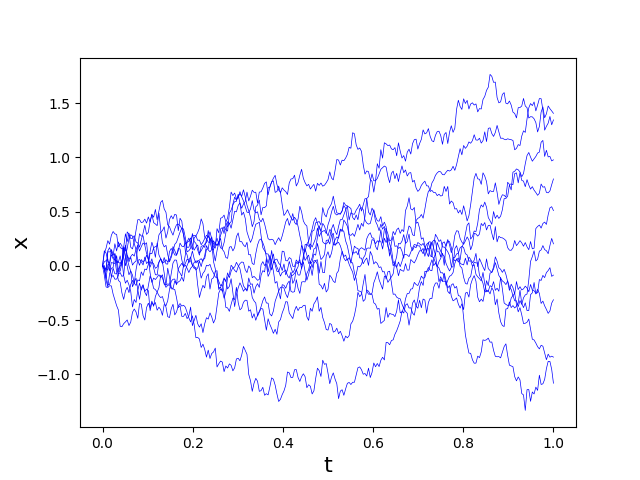
\includegraphics[scale=0.6]{content/Graphics/Figure_SamplingWienerProcess.png}
  \caption{10 realisations of discretizations of the Wiener process with n = 256 on [0,1].}
  \label{fig:fig1}
\nopagebreak
\end{figure}	

\begin{samepage}
To get a refinement for a given discrete sample path, we can use the following procedure. As an input we give a realisation of a discrete sample path \((\overline{W}_{t_0},\dots, \overline{W}_{t_n})\), n steps with step size \(\delta\). The output is a sample from the same process but with 2n steps: \(\left(\overline{W}_{R,t_0},\dots,\overline{W}_{R,t_n}\right)\), which makes a step size of \(\frac{\delta}{2}\).
We can use this procedure recursively to get finer and finer sample paths and imitate the convergence stated above.\footnote{See also Paul L\'evy's construction of the Wiener process in \cite{BMIntro} which follows the same idea.}
\begin{algorithm}[Refinement of a given discretized Wiener sample path]
\label{alg:Refinement}
\begin{enumerate}[noitemsep,topsep=0mm,labelindent=6mm,leftmargin=*,widest=3.,align=right]
\item For j = 0 to n-1
\begin{enumerate}[noitemsep,topsep=0mm,labelindent=6mm,leftmargin=*,widest=3.,align=right]
\item Generate \(z\sim \mathcal{N}(\frac{\overline{W}_{(j+1)\delta}+\overline{W}_{j\delta}}{2}, \frac{\delta}{4})\)
\item Set \(\overline{W}_{R,j\delta} = \overline{W}_{j\delta}\)
\item Set \(\overline{W}_{R,(j+\frac{1}{2})\delta} = z\)
\end{enumerate}
\item Set \(\overline{W}_{R,n\delta} = \overline{W}_{n\delta}\)
\item Linear interpolation.
\end{enumerate}
\end{algorithm}
This algorithm follows from the fact that \(W_{(j+\frac{1}{2})\delta}\mid_{ \!W_{j\delta}=a,\! W_{(j+1)\delta}\!=b} \sim \mathcal{N}({\frac{a+b}{2}}, \frac{\delta}{4})\).
\begin{figure}[!h]
\centering
  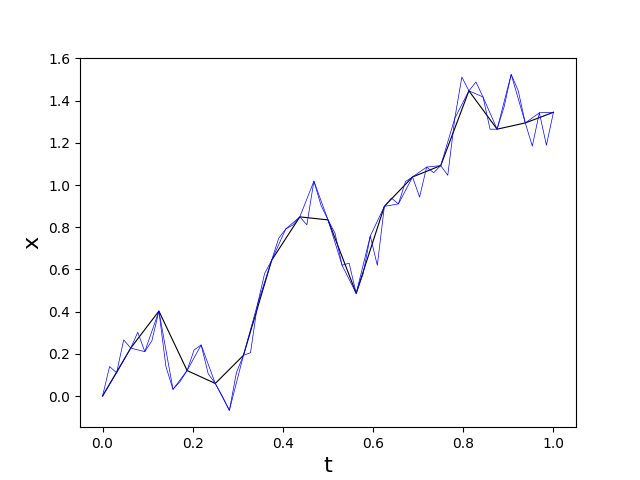
\includegraphics[scale=0.6]{content/Graphics/Figure_RefinementPath2.png}
  \caption{Finer versions of a given discretized Wiener process (black).}
  \label{fig:fig2}
\end{figure}
\end{samepage}
\section{Stochastic integration: It\^o and Stratonovich}
\label{sec:StochInt}
In this section we will present 2 (of many other possible) definitions of the stochastic integral for a basic example. We will show that both definitions yield different values.
Both definitions lead to 2 different stochastic calculii, the first one being called \emph{It\^o -} the second one \emph{Stratonovich stochastic calculus}.
In the next chapter (and in the rest of this thesis) we will focus on the definition due to It\^o and it will become clear, why this definition is more practical.


Our first attempt on defining the stochastic integral will be for the following example: 
\[\int_0^T \! 2W_t \, \mathrm{d}W_t.\]
The idea is to construct a partition of [0,T] and to evaluate the function only on these countable amount of time intervals, similar to Riemann(-Stieltjes)-sum approximation in the discrete case.
Then we take the limit of this sum and check for convergence in the \(L^2[\Omega]\)-norm.
Thus the stochastic integral will be defined as a limit of a sum of random variables and is thus also a random variable on the same probability space, if it exists\footnote{The limit of a sequence of measurable functions remains measurable, if it exists.}.
The limiting value will depend on which point on the intervals we evaluate the function. This is a counter-intuitive fact which does not hold in the deterministic case. If we evaluate the function at the start of each time interval, e.g. at \(t_j\) for \([t_j,t_{j+1}]\), we get the \emph{It\^o stochastic integral} and if we evaluate it at \(t_{j+\frac{1}{2}}\), at the middle of each time interval, we get the \emph{Stratonovich stochastic integral}.
\begin{definition}[Riemann-sum approximation]
Let \(P_n\) be a partition of [0,T], where n denotes the amount of steps. For our purposes we will consider only constant step sizes \(\delta\), e.g. \(P_n\coloneqq \{t_0 = 0, \dots, t_n = n\delta = T\}\) where T is fixed and \(\delta\) depends on n.
\begin{flalign*}
 R_{1,n} \coloneqq  R_1(P_n) &\coloneqq \sum_{k=0}^{n-1}2W_{t_k}\Delta W_{t_k}				  \tag{It\^o}  \\
 R_{2,n} \coloneqq  R_2(P_n) &\coloneqq \sum_{k=0}^{n-1}2W_{t_{k+\frac{1}{2}}}\Delta W_{t_k}   \tag{Stratonovich}
\end{flalign*}
where \(\Delta W_{t_k}\coloneqq W_{t_{k+1}}-W_{t_k}\) and \(W_{t_{k+\frac{1}{2}}}\) is the value of the process taken in the center of the interval [\(t_k, t_{k+1}\)].
\end{definition}
The key question which arises is whether \(R_{1,n}\) and \(R_{2,n}\) converge (in \(L^2[\Omega]\)) as n goes to infinity (e.g. \(\delta\) goes to 0). 
Indeed, using the proposition on quadratic variation which we will present later, we can show that the limits exist, but are not identical:
\begin{lemma}[Stochastic integration of \(\int_0^T \! 2W_t \, \mathrm{d}W_t\)]
\label{lemma:StochInt}
Let \(P_n\) be a partition of [0,T]. Then
\begin{flalign*}
 R_{1,n} &\rightarrow W_T^2 - T \quad  (\text{in } L^2[\Omega])\text{ as }n\to\infty \tag{It\^o} \\
 R_{2,n} &\rightarrow W_T^2 \quad       (\text{in } L^2[\Omega])\text{ as }n\to\infty \tag{Stratonovich}
\end{flalign*}
Notice also that \(W_T^2-T\) is a well-known martingale and \(W_T^2\) is what we would get in the deterministic case.
\end{lemma}
In order to calculate this, we need the following proposition:
\begin{proposition}[Quadratic variation]
Let \(P_n\) be a partition of [0,T]. Note that the step size \(\delta \rightarrow 0\) as \(n\rightarrow \infty\). Then
\[\sum^{n-1}_{k=0}(W_{t_{k+1}}-W_{t_{k}})^2 \rightarrow T \text{ as }n\rightarrow\infty\qquad(\text{in } L^2[\Omega]).\]
This implies the heuristic \((dW_t)^2=dt\) which is often seen in literature on stochastic calculus.
\end{proposition}
\begin{proof}
We will use the independence property of the Wiener process.
\begin{flalign*}
& \mathbb{E}[(\sum^{n-1}_{k=0}(W_{t_{k+1}}-W_{t_{k}})^2-T)^2] = \mathbb{E}[(\sum^{n-1}_{k=0}((W_{t_{k+1}}-W_{t_{k}})^2-\frac{T}{n}))^2]\\
& = \mathbb{E}[(\sum^{n-1}_{k=0}(x_k^2-\frac{T}{n}))^2] = \sum^{n-1}_{k,j=0}\mathbb{E}[(x_k^2-\frac{T}{n})(x_j^2-\frac{T}{n})]\\ 
& (\text{where }W_{t_{k+1}}-W_{t_{k}}\coloneqq x_k\sim\mathcal{N}(0,\frac{T}{n}))\\ 
& = \sum^{n-1}_{l=0}\mathbb{E}[(x_k^2-\frac{T}{n})^2] = \sum^{n-1}_{l=0}\text{Var}[x_k^2-\frac{T}{n}] + \underbrace{\mathbb{E}[x_k^2-\frac{T}{n}]^2}_{= 0}\\ 
& = \sum^{n-1}_{l=0}\textnormal{Var}[x_k^2] = 2n(\frac{T}{n})^2\rightarrow 0\text{ as }n\rightarrow\infty.
\end{flalign*}
\end{proof}
Now we are able to show lemma \ref{lemma:StochInt}.
\begin{proof}
We will show the lemma only for the It\^o-case:
\begin{flalign*}
& \mathbb{E}[(\sum^{n-1}_{k=0}2W_{t_{k}}(W_{t_{k+1}}-W_{t_{k}})-(W_T^2-T))^2] \\
& = \mathbb{E}[(\sum^{n-1}_{k=0}(W_{t_{k+1}}^2-W_{t_{k}}^2)-(W_{t_{k+1}}-W_{t_{k}})^2-(W_T^2-T))^2]\\
& (\text{Where we used that } 2X(Y-X) = (Y^2-X^2)-(X-Y)^2,\quad X\coloneqq W_{t_{k}}, Y\coloneqq W_{t_{k+1}})\\
& = \mathbb{E}[(\sum^{n-1}_{k=0}-(W_{t_{k+1}}-W_{t_{k}})^2+T)^2]\\
& = \mathbb{E}[(\sum^{n-1}_{k=0}(W_{t_{k+1}}-W_{t_{k}})^2-T)^2] \rightarrow 0, \text{ as }n\rightarrow\infty\ \\
& \text{using quadratic variation.}\quad\qquad
\end{flalign*}
\end{proof}
Is it possible to take other integrands than just \(2W_t\)?
In the next chapter we will give the idea behind the construction of the It\^o stochastic integral for a class of functions \(\mathcal{C}\) and we will give an argument on why we choose the definition of It\^o over the definition of Stratonovich.
\chapter{It\^o Stochastic Calculus}
\label{ch:ItoCalc}
In this section we will give the idea behind the construction of the stochastic integral in the It\^o-sense for a certain class of functions \(\mathcal{C}\).
We will also present the fundamental theorem of stochastic calculus, namely \emph{It\^o's lemma}, and give examples. Later we will discuss an important application of this lemma, the so-called \emph{stochastic Taylor expansion} (or \emph{Wagner-Platen expansion}). We will use it to construct our numerical schemes which we will discuss in chapter \ref{ch:Num}.
\section{Construction of the It\^o stochastic integral}
We want to define:
\[\int_0^T \! X_t \, \mathrm{d}W_{t}\]
for a large class of functions \(X_t\in\mathcal{C}(0,T)\), \(X_t\!:[0,T]\!\times\Omega\rightarrow\mathbb{R}\).

First let us define the space of square-integrable stochastic processes:
\[L^{2}[0,T] \coloneqq \{X_t\!: [0,T]\times\Omega \rightarrow \mathbb{R}\mid X_t \text{ measurable},\, \mathbb{E}[\int^{T}_{0}X_t^2\mathrm{d}t]<\infty\}.\]
If we interpret the second condition as norm, we get the \emph{complete normed space} \((L^{2}[0,T], \|\cdot\|_{L^2[0,T]})\).
However we want to exclude functions from this class which are not \(\mathcal{F}_t\)-adapted.
Let us consider now the subset \(\mathcal{C}\coloneqq\mathcal{C}[0,T]\) of all functions \(X_t\) in \(L^{2}[0,T]\) which are adapted.
A limit of a sequence of adapted processes remains adapted\footnote{See \cite{BMKaratzas} for the proof.}. Thus \(\mathcal{C}\) is a closed subset of \(L^2[0,T]\) since it includes all its limits, which implies that \(\mathcal{C}\) is also complete under the same norm. Thus we have the complete normed space \((\mathcal{C}, \|\cdot\|_{L^2[0,T]})\). Recall that we want to define the It\^o stochastic integral for functions in \(\mathcal{C}\). 
First we will define the stochastic integral for a simpler class of functions \(\mathcal{E}\), s.t \(\mathcal{E}\subset\mathcal{C}\), and then expand the definition to the space \(\mathcal{C}\).

Define the space of \emph{random step functions} \(\mathcal{E}\) which can be expressed in the following form:
\[\xi_t^{n} = \sum^{n-1}_{k=0}Z_k\cdot\mathbb{1}_{[t_k,t_{k+1})}\]
for a partition \(P_n\) of [0,T] and some random variables \(Z_k \:\:\mathcal{F}_{t_k}\)-measurable and square-integrable (this means \(Z_k\) is in \(L_2[\Omega]\)) for \(k\!=\!0,\dots,\! n\!-\!1\).
Obviously \(\xi_t^{n}\) is \(\mathcal{F}_t\)-adapted and \(\mathcal{E}\subset\mathcal{C}\).
\begin{definition}[It\^o stochastic integral for random step functions]
Let \(\xi_t^{n}\!\in\mathcal{E}\) be a random step function with the above representation. Then 
\begin{displaymath}
\int_0^T \! \xi_t^{n}\, \mathrm{d}W_{t}\coloneqq\sum^{n-1}_{k=0}Z_k\cdot(W_{t_{k+1}}-W_{t_{k}})
\end{displaymath}
is the It\^o stochastic integral of \(\xi_t^{n}\). Note that the integral is a random variable and \(\mathcal{F}_T\)-measurable. If we allow the upper limit of the integral to be in the intervall [0,T], then the It\^o stochastic integral becomes an adapted
stochastic process. This would not be true in the Stratonovich calculus or if \(X_t\) were not adapted.
\end{definition}
For \(X_t\in\mathcal{C}\) we have the construction \(\xi_t^{n}=\sum^{n-1}_{k=0}X_{t_k}\cdot\mathbb{1}_{[t_k,t_{k+1})}\) which is also adapted. 

\begin{figure}[!h]
\centering
  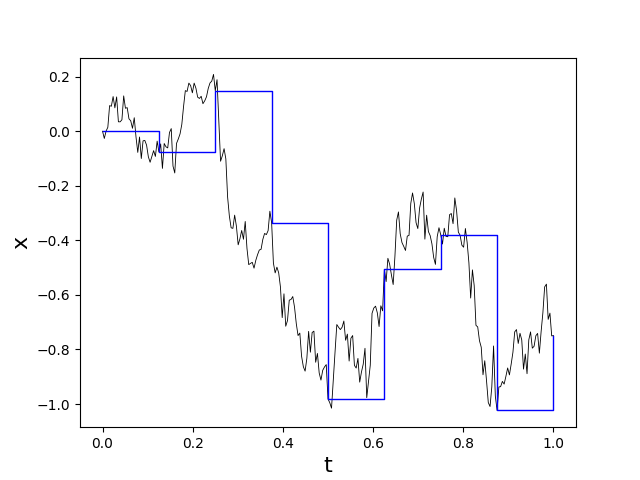
\includegraphics[scale=0.6]{content/Graphics/Figure_WienerStepProcess.png}
  \caption{A sample of the Wiener process and its corresponding step function  for n = 8.}
  \label{fig:fig3}
\nopagebreak
\end{figure}	
The following result will be important for our construction of It\^o stochastic integrals for functions in \(\mathcal{C}\):
\begin{proposition}[It\^o-isometry for random step functions]
Let \(\xi_t\!\in\mathcal{E}\). Then
\begin{align*}
\mathbb{E}[(\int_0^T\!\xi_t\,\mathrm{d}W_{t})^2] = \mathbb{E}[\int_0^T\!(\xi_t)^2\,\mathrm{d}t]\\
\|\int_0^T\!\xi_t\,\mathrm{d}W_{t}\|_{L^2[\Omega]} = \|\xi_t\|_{L^2[0,T]}.
\end{align*}
We conclude that for all \(\xi_t\in\mathcal{E}\) there exists \(\int_0^T\!\xi_t\,\mathrm{d}W_{t}\) as an element in \({L^2[\Omega]}\).
\end{proposition}
\begin{proof}
\begin{flalign*}
& \mathbb{E}[(\int_0^T\!\xi_t\,\mathrm{d}W_{t})^2]  \\
&= \mathbb{E}[(\sum^{n-1}_{k=0}Z_k\cdot(W_{t_{k+1}}-W_{t_{k}}))(\sum^{n-1}_{l=0}Z_l\cdot(W_{t_{l+1}}-W_{t_{l}}))] \\
&= \mathbb{E}[\sum^{n-1}_{k=0}Z_k^2\cdot(W_{t_{k+1}}-W_{t_{k}})^2] + 2\mathbb{E}[\sum^{n-1}_{k>l=0}Z_k\cdot Z_l\cdot(W_{t_{k+1}}-W_{t_{k}})(W_{t_{l+1}}-W_{t_{l}})] \\
&= \sum^{n-1}_{k=0}\mathbb{E}[Z_k^2]\cdot\mathbb{E}[(W_{t_{k+1}}-W_{t_{k}})^2]\\
& \text{Where we used that \(Z_k^2\), \((W_{t_{k+1}}-W_{t_{k}})^2\)  and \(Z_l\cdot(W_{t_{k+1}}-W_{t_{k}})(W_{t_{l+1}}-W_{t_{l}})\), \(Z_k\)}\\
& \text{are independent for } k>l. \\
& \sum^{n-1}_{k=0}\mathbb{E}[Z_k^2]\cdot(t_{k+1}-t_{k}) = \mathbb{E}[\int_0^T\!(\xi_t)^2\,\mathrm{d}t]
\end{flalign*}
\end{proof}
The proof would not be possible in case of the Stratonovich calculus or if \(X_t\) were not adapted. For example if \(X_t = W_{t+\frac{1}{2}}\).

Finally, using the following lemma, we can expand our definition of the stochastic integral from \(\mathcal{E}\) to \(\mathcal{C}\):
\begin{lemma}[It\^o stochastic integral]
Let \(X_t\in\mathcal{C}\). Then there exists a sequence \(({\xi_{t}^n})_{n\!\in\!\mathbb{N}}\in\mathcal{E}\) s.t.
\(\mathbb{E}[\int_{0}^{T}(X_t-\xi_{t}^n)^2\mathrm{d}t] = \|X_t-\xi_{t}^n\|^2_{L^2[0,T]}\rightarrow 0\:\text{as}\:n\rightarrow\infty\) and 
\begin{align*}
\int_{0}^{T}\xi_t^n\mathrm{d}W_t\rightarrow\int_{0}^{T}X_t\mathrm{d}W_t\quad(\text{in}\:L^2[\Omega])\:\:\text{as}\:n\rightarrow\infty.
\end{align*}
This means \(\|\int_{0}^{T}X_t\mathrm{d}W_t-\int_{0}^{T}\xi_t^n\mathrm{d}W_t\|_{L^2[\Omega]} \rightarrow 0\:\:\text{as}\:n\rightarrow\infty.\)
And we can define:
\[\int_0^T\! X_t\,\mathrm{d}W_{t} \coloneqq\lim_{n\to\infty}\int_0^T\! \xi_t^n\,\mathrm{d}W_{t}  \:\:(\text{in}\:L^2[\Omega]).\]
Additionaly, the It\^o-isometry holds also in \(\mathcal{C}\).
\end{lemma}

The idea of the construction is to show that \(\mathcal{E}\) is dense in \(\mathcal{C}\) w.r.t the norm \(\|\cdot\|_{L^2[0,T]}\) using an approximation procedure, see \cite{Oksendal} for the details.
This means there exists a sequence \((\xi_t^n)_{n\!\in\!\mathbb{N}}\in\mathcal{E} \text{ s.t. } \|X_t-\xi_t^n\|_{L^2[0,T]}\rightarrow 0 \text{ as } n\rightarrow\infty\:\:\forall\: X_t\in\mathcal{C}\).
Since \( L^2[0,T]\) is complete, \(({\xi_t^n})_{n\!\in\!\mathbb{N}}\) is a Cauchy-sequence in this space. Using the It\^o-isometry, we then have:
\[\|\xi_t^n-\xi_t^m\|_{L^2[0,T]} = \|\int_{0}^{T}\xi_t^n\mathrm{d}W_t-\int_{0}^{T}\xi_t^m\mathrm{d}W_t\|_{L^2[\Omega]}\rightarrow 0 \text{ as } n,m\rightarrow\infty.\]
Hence \(({\int_{0}^{T}\xi_t^n}\mathrm{d}W_t)_{n\!\in\!\mathbb{N}}\) is a Cauchy-sequence in \(L^2[\Omega]\). It is well known that this space is complete\footnote{\(L^2[\Omega]\) is the usual space of square-integrable random variables on
\(\left( \Omega , \mathcal{F}, P\right)\).}. 
Thus, it makes sense to define:
\[\int_0^T\! X_t\,\mathrm{d}W_{t} \coloneqq\lim_{n\to\infty}\int_0^T\! \xi_t^n\,\mathrm{d}W_{t} \quad(\text{in }L^2[\Omega])\]
as an element in \(L^2[\Omega]\).

 
We still need to clarify why we choose It\^o over Stratonovich. As can be seen, the definition due to It\^o simplifies our calculations and enables us to define the stochastic integral in a straightforward way through the isometry. The isometry does not hold in the Stratonovich calculus. Additionaly we are able to identify the It\^o stochastic integral as a martingale\footnote{See \cite{Oksendal} for the interpretation of It\^o stochastic integrals as martingales. The expected value of the It\^o stochastic integral is always 0 and the It\^o stochastic integral can be defined as adapted stochastic process.}.


\section{Lemma of It\^o}
\label{itolemma}
The lemma of It\^o enables us to evaluate stochastic integrals without using the definition as in section \ref{lemma:StochInt}. 
Given a stochastic process \(X_t\) and its representation as stochastic integral equation, we may ask, what is the representation of \(u(X_t)\) where u:\(\mathbb{R}\to\mathbb{R}\) is a smooth map? 
We will present the lemma of It\^o in 3 cases: In the first case, \(X_t=W_t\) and we are interested in \(u(W_t)\). Then we will consider more general stochastic processes \(X_t\). Finally we will allow the mapping u:\(\mathbb{R}\times[0,T]\to\mathbb{R}\) to depend on the paramter t.
\begin{definition}[It\^o process]
\label{Itoprocess}
We will call a stochastic process \(X_t\) an It\^o process if it has a known representation as stochastic integral equation of the following form:
\[X_t - X_0 = \int_0^t \!a(X_s,s)\,\mathrm{d}s + \int_0^t \!b(X_s,s)\,\mathrm{d}W_{s}\]
where \(b(X_t,t)\in\mathcal{C},\:\: a(X_t,t)\: \mathcal{F}_t\)-adapted and \(\mathbb{E}[\int_{0}^{T}(a(X_t,t))^2\mathrm{d}t]<\infty\). \\
Then \(X_t\in L_2[\Omega]\) \(\forall\; t\in[0,T]\) fixed and we have the (symbolical) differential form:
\[\mathrm{d}X_t = a(X_t,t)\mathrm{d}t + b(X_t,t)\mathrm{d}W_t.\]
We will only consider the autonomous case where the functions \(a(x,t) \equiv a(x)\) and \(b(x,t) \equiv b(x)\) do not depend on the additional parameter t.

\end{definition}
\begin{lemma}[It\^o lemma for the Wiener process]
Let \(W_t\) be the Wiener process. Let u:\(\mathbb{R}\to\mathbb{R}\) be twice continuously differentiable with derivatives \(u_x(x), u_{xx}(x)\). Define \(Y_t \coloneqq u(W_t)\). Then
\begin{displaymath}
Y_t-Y_0 = \int_0^t \!\frac{1}{2}u_{xx}(W_s)\,\mathrm{d}s + \int_0^t \!u_x(W_s)\,\mathrm{d}W_{s}
\end{displaymath}
where equality is P-a.s. for \(t\in[0,T]\).
\end{lemma}
\begin{proof}
Proof follows from the general case, lemma \ref{lemma:ito}, and by using that \(W_t = \int_0^t \!\,\mathrm{d}W_{s}\).
\end{proof}
\begin{lemma}[It\^o lemma, non time-dependent case]
Let \(X_t\) be an It\^o process. 
Let u:\(\mathbb{R}\to\mathbb{R}\) be twice continuously differentiable with derivatives \(u_x(x), u_{xx}(x)\). Define \(Y_t \coloneqq u(X_t)\). Then
\begin{displaymath}
Y_t-Y_0  = \int_0^t \!u_x(X_s)a(X_s) + \frac{1}{2}u_{xx}(X_s)b(X_s)^2\,\mathrm{d}s + \int_0^t \!u_x(X_s)b(X_s)\,\mathrm{d}W_{s} 
\end{displaymath}
where equality is P-a.s. for \(t\in[0,T]\).
\end{lemma}
\begin{proof}
See general case.
\end{proof}
\begin{lemma}[It\^o lemma, general case]
\label{lemma:ito}
Let \(X_t\) be an It\^o process. 
Let u:\(\mathbb{R}\times[0,T]\to\mathbb{R}\) be twice continuously differentiable with partial derivatives \(u_x(x,t), u_{xx}(x,t)\) and \(u_t(x,t)\). Define \(Y_t \coloneqq u(X_t,t)\).  Then
\begin{flalign*}
Y_t-Y_0  = & \int_0^t \!u_t(X_s,s)+u_x(X_s,s)a(X_s)\:\: + \\
		    & \frac{1}{2}u_{xx}(X_s,s)b(X_s)^2\,\mathrm{d}s + \int_0^t \!u_x(X_s,s)b(X_s)\,\mathrm{d}W_{s} 
\end{flalign*}
where equality is P-a.s. for \(t\in[0,T]\).
\end{lemma}
\begin{proof}
See \cite{Oksendal}.
\end{proof}
Let us consider some examples:
\begin{example}
Let \(X_t=W_t\) and u: \(x\mapsto x^2\). Then
\begin{flalign*}
& W_t^2 = \int_0^t \!\,\mathrm{d}s + \int_0^t \!2W_s\,\mathrm{d}W_{s}\\
& W_t^2 - t =  \int_0^t \!2W_s\,\mathrm{d}W_{s}\quad\text{by rearrangement.}
\end{flalign*}
This is the same result as in lemma \ref{lemma:StochInt} where we used the definition to calculate this stochastic integral in the It\^o sense.
\end{example}

\begin{example}
\label{ex:gbm}
Let \(X_t - X_0 = \int_0^t \!\mu X_s\,\mathrm{d}s + \int_0^t \!\sigma X_s\,\mathrm{d}W_{s}\). \(\mu,\:\sigma>0\) constants\\
and u: \(x\mapsto\ln(x)\: (x\neq 0)\). Then
\begin{flalign*}
& u_x(x) = \frac{1}{x}\:\:\text{ and }\:\:u_{xx}(x) = -\frac{1}{x^2} \\
u(X_t)-u(X_0) & = \int_0^t \!u_x(X_s)\mu X_s + \frac{1}{2}u_{xx}(X_s)(\sigma X_s)^2\,\mathrm{d}s + \int_0^t \!u_x(X_s)\sigma X_s\,\mathrm{d}W_{s} \\
			  & = \int_0^t \!\mu - \frac{1}{2}\sigma^2\,\mathrm{d}s + \int_0^t \!\sigma\,\mathrm{d}W_{s} = (\mu - \frac{1}{2}\sigma^2)t + \sigma W_t.\\
\end{flalign*}
This just means: 
\[\ln{X_t} = \ln{X_0} + (\mu - \frac{1}{2}\sigma^2)t + \sigma W_t\]
where \(X_0\) can be set as an initial value (can be a random variable under some conditions).
This example will be of importance in the next chapter.
\end{example}
\section{Stochastic Taylor expansions}
 \label{stochasticTaylor}

Given a deterministic and smooth function \(X(t)\) and \(\frac{\mathrm{d}}{\mathrm{d}t}X(t) = a(X(t))\) we can express it using the fundamental theorem of calculus as:
\[X(t)-X(0) = \int_0^t \!a(X(s))\,\mathrm{d}s.\]
We can reapply the theorem on \(a(X(s))\) and use the chain rule to get:
\begin{flalign*}
X(t)-X(0) & = \int_0^t \!a(X(0))\,\:+\,\:\int_0^s \!a^{\prime}(X(r))\cdot a(X(r))\,\mathrm{d}r\,\mathrm{d}s\\
		 & = a(X(0))t\,\:+\int_0^t\!\int_0^s \!a^{\prime}(X(r))\cdot a(X(r))\,\mathrm{d}r\,\mathrm{d}s.
\end{flalign*}
Indeed we could show this representation using the Taylor expansion and by plugging in the derivative of \(X(t)\).

The second integral is of quadratic order (\(\mathcal{O}(t^2)\)) (Where we assumed that the derivatives are bounded). If we truncate the second integral we can give a linear approximation of X(t) for t small, where \(x_0=X(0)\) is a given initial value.
This is the simplest approximation for (deterministic) ordinary differential equations, the so-called \emph{explicit Euler-scheme}.

We want to construct similar approximation schemes in the stochastic setting.
Let \(X_t\) be a stochastic process and its representation as It\^o process, where a:\(\mathbb{R}\to\mathbb{R}\), b:\(\mathbb{R}\to\mathbb{R}\) are smooth and have bounded derivatives (see \ref{Itoprocess}):
\[X_t - X_0 = \int_0^t \!a(X_s)\,\mathrm{d}s + \int_0^t \!b(X_s)\,\mathrm{d}W_{s}.\]
Later we will call such equations \emph{stochastic differential equations}, where \(X_0=x_0\) is a (possibly random) initial value.\\
Applying the lemma of It\^o on \(a(X_s)\) and \(b(X_s)\) gives us:
\[a(X_s) = a(X_0) + \int_0^s \!a_x(X_r)a(X_r) + \frac{1}{2}a_{xx}(X_r)b(X_r)^2\,\mathrm{d}r + \int_0^s \!a_x(X_r)b(X_r)\,\mathrm{d}W_{r}\]
\[b(X_s) = b(X_0) + \int_0^s \!b_x(X_r)a(X_r) + \frac{1}{2}b_{xx}(X_r)b(X_r)^2\,\mathrm{d}r + \int_0^s \!b_x(X_r)b(X_r)\,\mathrm{d}W_{r}\]
and by plugging in to the original equation we get:
\begin{flalign*}
X_t - X_0 = & \int_0^t \! a(X_0) + \int_0^s \!a_x(X_r)a(X_r) + \frac{1}{2}a_{xx}(X_r)b(X_r)^2\,\mathrm{d}r + \int_0^s \!a_x(X_r)b(X_r)\,\mathrm{d}W_{r}\,\mathrm{d}s\\
		+   &\int_0^t \!b(X_0) + \int_0^s \!b_x(X_r)a(X_r) + \frac{1}{2}b_{xx}(X_r)b(X_r)^2\,\mathrm{d}r + \int_0^s \!b_x(X_r)b(X_r)\,\mathrm{d}W_{r}\,\mathrm{d}W_{s}
\end{flalign*}
This means:
\begin{flalign*}
 X_t = X_0 & +  \int_0^t \! a(X_0)\,\mathrm{d}s + \int_0^t \!\int_0^s \!a_x(X_r)a(X_r) + \frac{1}{2}a_{xx}(X_r)b(X_r)^2\,\mathrm{d}r\,\mathrm{d}s\\
		    &	 +  \int_0^t \!\int_0^s \!a_x(X_r)b(X_r)\,\mathrm{d}W_{r}\,\mathrm{d}s\\
	    	    & +  \int_0^t \! b(X_0)\,\mathrm{d}W_{s} + \int_0^t \!\int_0^s \!b_x(X_r)a(X_r) + \frac{1}{2}b_{xx}(X_r)b(X_r)^2\,\mathrm{d}r\,\mathrm{d}W_{s}\\
		    &	 +  \int_0^t \!\int_0^s \!b_x(X_r)b(X_r)\,\mathrm{d}W_{r}\,\mathrm{d}W_{s}
\end{flalign*}
This gives us the simplest \emph{stochastic Taylor expansion}:
\begin{proposition}[1. stochastic Taylor expansion]
\label{prop:stochTaylor1}
Given the It\^o process \(X_t\) as above. Then
\begin{flalign*}
 X_t-X_0  & =  \int_0^t \!a(X_0)\,\mathrm{d}s +  \int_0^t \!b(X_0)\,\mathrm{d}W_{s} + R \\
		  & = a(X_0)t + b(X_0)W_t + R
\end{flalign*}
where R is the remainder term, containing in this case integrals of order t and above.
\end{proposition}
Note that integrals of the form \(\int_0^t \!\int_0^s \!\,\mathrm{d}W_{r}\,\mathrm{d}s\) have higher order than t \mbox{(in \(L^2[\Omega]\)).}
More important: We can give an estimate for the last integral in the remainder term: 
\[\mathbb{E}[(\int_0^t \!\int_0^s \!b_x(X_r)b(X_r)\,\mathrm{d}W_{r}\,\mathrm{d}W_{s})^2]^{\frac{1}{2}} = \mathbb{E}[\int_0^t \!\int_0^s \!(b_x(X_r)b(X_r))^2\,\mathrm{d}r\,\mathrm{d}s]^\frac{1}{2} = \mathcal{O}(t).\]
Where we used the boundedness of b and its derivative and the It\^o-isometry twice.

The above expansion is insofar discrepant as it contains integrals of order t in both, the main term and the remainder term. This is not true in the deterministic case.
However we can reapply the It\^o lemma on \(b_x(X_r)b(X_r)\) and plug it into the above equation. This gives us the second \emph{stochastic Taylor expansion}:
\begin{proposition}[2. stochastic Taylor expansion]
\label{prop:stochTaylor2}
Given the It\^o process \(X_t\) as above. Then
\begin{flalign*}
X_t-X_0  & =  \int_0^t \!a(X_0)\,\mathrm{d}s +  \int_0^t \!b(X_0)\,\mathrm{d}W_{s} + \int_0^t \!\int_0^s \!\,b_x(X_0)b(X_0)\mathrm{d}W_{r}\,\mathrm{d}W_{s} + R \\
		 & = a(X_0)t + b(X_0)W_t + \frac{1}{2}b_x(X_0)b(X_0)(W_t^2-t) +  R
\end{flalign*}
where R is the remainder term, containing in this case integrals of order strictly higher than t.
\end{proposition}
Through iterative usage of the It\^o lemma we got an expansion which can be seen as a generalization of the Taylor expansion from deterministic calculus. Taylor expansions can be used to construct numerical schemes for ordinary differential equations.
In the next chapter we will define stochastic differential equations as It\^o processes and in chapter \ref{ch:Num} we will use stochastic Taylor expansions to construct numerical schemes for stochastic differential equations.





\chapter{Stochastic Differential Equations}
\label{ch:SDE}
In this chapter we will define what we mean when we say that \(X_t\) is a \emph{solution} (or \emph{solution process}) of a stochastic differential equation and we will discuss the conditions under which the solution exists and its uniqueness. Furthermore we will give some examples of stochastic differential equations which can be solved analytically.
\section{Existence and uniqueness of solutions}
\begin{definition}[Stochastic differential equation]
Let a:\(\mathbb{R}\times[0,T]\to\mathbb{R}\) and b:\(\mathbb{R}\times[0,T]\to\mathbb{R}\) be measurable functions.
A stochastic differential equation (SDE) has the following form:
\begin{flalign*}
\text{SDE}\quad\begin{cases} \mathrm{d}X_t = a(X_t,t)\mathrm{d}t + b(X_t,t)\mathrm{d}W_t \\ 
X_0 = x_0\:\:\text{(initial value)}  \\
\end{cases}
\end{flalign*} 
for \(t\in[0,T]\). We will give it the following (It\^o-)representation:
\[X_t = x_0 + \int_0^t \!a(X_s,s)\,\mathrm{d}s + \int_0^t \!b(X_s,s)\,\mathrm{d}W_{s} \quad\text{P-a.s.}\]
and the following has to hold:
\begin{enumerate}[noitemsep,topsep=0mm,labelindent=6mm,leftmargin=*,widest=3.,align=right]
\item \(x_0\) is \(\mathcal{F}_0\)-measurable and \(\mathbb{E}[|x_0|^2]<\infty\:\:\)(can be constant). 
\item \(a(X_t,t)\) and \(b(X_t,t)\) as in definition \ref{Itoprocess}.
\end{enumerate}
\end{definition}
\begin{lemma}[Existence and Uniqueness]
\label{lemma:ExUn}
Given a stochastic differential equation as before. The solution \(X_t\) exists and is unique (P-a.s) if there are constants C, L \(\in\mathbb{R}\) s.t:
\begin{enumerate}[noitemsep,topsep=0mm,labelindent=6mm,leftmargin=*,widest=3.,align=right]
\item \(|a(x,t) - a(y,t)| \leq L|x-y| \\
	    |b(x,t) - b(y,t)| \leq L|x-y|\:\: \forall x,y\in\mathbb{R}, t\in[0,T] \:\:\text{(globally Lipschitz)} \) 	
\item \(|a(x,t)| \leq C(1+|x|) \\
	    |b(x,t)| \leq C(1+|x|)\:\:  \forall x\in\mathbb{R}, t\in[0,T] \:\:\text{(linear growth-bound)}\)
\end{enumerate}
In the autonomous case, where \(a(x,t) = a(x)\) and \(b(x,t) = b(x)\), the Lipschitz-condition implies the second condition.
\end{lemma}
\begin{proof}
See \cite{Oksendal}.
\end{proof}
\section{Analytically solvable equations}
There are not many stochastic differential equations which have an analytical (closed-form) solution. We will present the \emph{geometric Brownian motion} and the \emph{Ornstein-Uhlenbeck process} which have applications in physics and mathematical finance. Both are solutions of stochastic differential equations.
Knowing the exact solution allows us to test how good our approximation schemes are using simulation. This will be the subject of chapter \ref{ch:Num}.
\label{sec:}
\subsection{Geometric Brownian motion}
\begin{proposition}[Geometric Brownian motion]
The stochastic differential equation is given by:
\begin{flalign*}
& \mathrm{d}X_t = \mu X_t\mathrm{d}t + \sigma X_t\mathrm{d}W_t,\quad t\in[0,T],\quad X_0 = x_0\\
& X_t = x_0 + \int_0^t \!\mu X_s\,\mathrm{d}s + \int_0^t \!\sigma X_s\,\mathrm{d}W_{s} \quad\text{P-a.s.}
\end{flalign*}
where \(x_0\), \(\mu\), \(\sigma\:\in\mathbb{R}\) constant and \(\sigma>0\).
Its solution is:
\[X_t = x_0\exp({(\mu-\frac{\sigma^2}{2})t + \sigma W_t}).\]
\end{proposition}
If we set \(x_0=1\), then \(X_t\sim\exp (Z_t)\) where \(Z_t\sim\mathcal{N}((\mu - \frac{1}{2}\sigma^2)t, \sigma^2 t)\). This means that \(X_t\) is lognormally distributed \(\forall\; t\in[0,T]\).
\begin{proof}
See example \ref{ex:gbm} and take the exponent. 
\end{proof}
\begin{figure}[!htbp]
\centering
  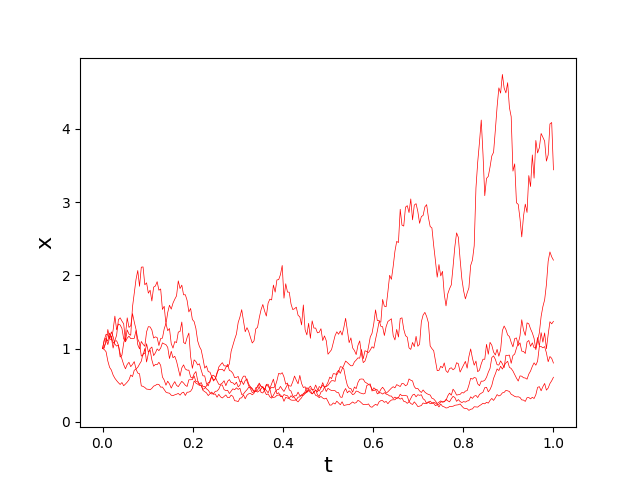
\includegraphics[scale=0.4]{content/Graphics/Figure_SamplingGBM.png}
  \caption{5 samples of the geometric Brownian motion with \(x_0 = 1, \mu = 1, \sigma = 1.5\).}
  \label{fig:}
\end{figure}

\subsection{Ornstein-Uhlenbeck process}
\begin{proposition}[Ornstein-Uhlenbeck process]
The stochastic differential equation is given by:
\begin{flalign*}
& \mathrm{d}X_t = -\beta X_t\mathrm{d}t + \sigma\mathrm{d}W_t,\quad t\in[0,T],\quad X_0 = x_0\\
& X_t = x_0 + \int_0^t \!-\beta X_s\,\mathrm{d}s + \int_0^t \!\sigma\,\mathrm{d}W_{s} \quad\text{P-a.s.}
\end{flalign*} 
where \(\beta\), \(\sigma\in\mathbb{R}\) constant and \(\beta\), \(\sigma>0\). We will choose \(x_0\) either to be constant or a normal-distributed random variable.
Its solution is:
\[X_t = x_0\exp({-\beta t}) + \sigma\int_0^t \!\exp({-\beta(t-s)})\,\mathrm{d}W_{s}.\]
\end{proposition} 
However we are not able to simulate the stochastic integral \(\int_0^{t_n} \!\,\exp({-\beta(t_n-s)})\,\mathrm{d}W_{s}\) exactly given the time step \(t_n\).
We will use the following approximation and consider it as the exact solution, given a partition \(P_n\) and a discretized Wiener process: 
\(\sum^{n-1}_{k=0}\exp({-\beta(t_n-t_k)})(W_{t_{k+1}}-W_{t_k})\).
\begin{proof}
Again we will use It\^o's lemma: Let u: \((x,t)\mapsto\ x\exp({\beta t})\). Then
\begin{flalign*}
& u_x(x,t) = \exp({\beta t}),      \:\:u_{xx}(x,t) = 0, \:\:u_{t}(x,t) =  x\beta\exp({\beta t})\\
& u(X_t,t)-u(X_0,0) = \int_0^t \!u_t(X_s,s) - \beta X_s\cdot u_x(X_s,s)  + \frac{1}{2}u_{xx}(X_s,s)\sigma^2\,\mathrm{d}s + \int_0^t \!\sigma u_x(X_s,s)\,\mathrm{d}W_{s} \\
& X_t\exp({\beta t}) - X_0\exp({\beta 0}) = \int_0^t \!\beta X_s\exp({\beta s}) - \beta X_s\exp({\beta s}) + 0 \,\mathrm{d}s + \int_0^t \!\sigma\exp({\beta s})\,\mathrm{d}W_{s} \\
%& X_t\exp({\beta t}) = x_0 + \int_0^t \!\sigma\exp({\beta s})\,\mathrm{d}W_{s} \\
& X_t =  x_0\exp({-\beta t}) + \sigma\int_0^t \!\exp({-\beta(t-s)})\,\mathrm{d}W_{s}.
\end{flalign*}
\end{proof}
\begin{figure}[H]
\centering
  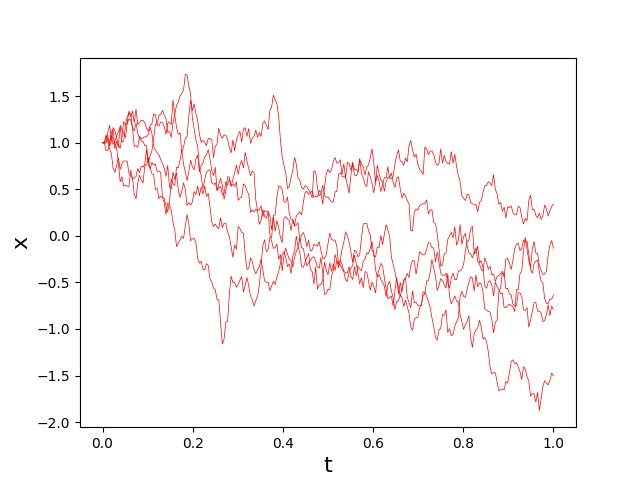
\includegraphics[scale=0.4]{content/Graphics/Figure_SamplingOU.png}
  \caption{5 samples of the Ornstein-Uhlenbeck process with \(x_0 = 1 , \beta = 1, \sigma = 1.5\).}
  \label{fig:}
\end{figure}



























\chapter{Numerical Analysis}
\label{ch:Num}
In this chapter we will discuss numerical methods for solving stochastic differential equations based on the stochastic Taylor expansions which have been presented in section \ref{stochasticTaylor}. These are also called \emph{time discrete approximations} since we will give the approximative values on points of the time interval [0,T]. We will consider strongly converging schemes only. Strong means in this context that we want to approximate the \emph{sample paths} of the true solution \(X_t\) of a stochastic differential equation. On the other hand, weakly converging schemes deal with the approximation of some funcionals of the true solution \(X_t\), for example the expected value or the variance. Obviously, strongly converging schemes are also weakly converging.\\
These methods will be discussed: \emph{Euler-Maruyama-scheme} and the \emph{Milstein-scheme}.\footnote{There is a third method which we also implemented: the \emph{Wagner-Platen-scheme}, but we will not give a discussion of this scheme and refer to \cite{KloedenPlaten} for the details, the scheme is also called \emph{order 1.5 strong stochastic Taylor scheme} and it is also based on the stochastic Taylor expansion. See appendix \ref{code} for the implementations and appendix \ref{Graphics} for graphics.}
We will prove the convergence of these methods and give the convergence order analytically. In the final sections of this chapter we will discuss the results and determine the convergence order numerically using simulations.


\section{Strong convergence and error analysis}
\label{erroranalysis}
For the moment, let us consider a general setting. Let \(X_t\) be the solution of a stochastic differential equation and let  \(\overline{X}_{t}\) denote its approximation on [0,T].  
We want that the sample paths on [0,T] of the approximation are close to the sample paths of the true solution (pathwise approximation).
There are many different criterions to measure the closeness or the approximation error:
\begin{enumerate}[noitemsep,topsep=0mm,labelindent=6mm,leftmargin=*,widest=3.,align=right]
\item \(\mathbb{E}[|X_T - \overline{X}_{T}|]\quad\) (absolute error at T)
\item \(\mathbb{E}[(X_T - \overline{X}_{T})^2]^{\frac{1}{2}}\quad\) (squared-mean error at T)
\item \(\sup_{t\in[0,T]}\mathbb{E}[|X_t - \overline{X}_{t}|]\quad\) (uniform absolute error)
\item \(\sup_{t\in[0,T]}\mathbb{E}[(X_t - \overline{X}_{t})^2]^{\frac{1}{2}}\quad\) (uniform squared-mean error)
\end{enumerate}
The first two criterions measure the error at the final time-point T. We will use the second criterion in our numerical simulations, since it is a bound for the absolute error at T: \(\mathbb{E}[|X_T - \overline{X}_{T}|]\leq\mathbb{E}[(X_T - \overline{X}_{T})^2]^{\frac{1}{2}}\) and the implementation is simple. We assume that the approximation error is determined at the final time point T. However we will use the uniform squared-mean error criterion in our convergence proofs.

Now let \(\overline{X}^{n}_{t}\) define a sequence of approximate solutions on partitions \(P_n\) of [0,T]. This means for each n we have a time-grid with n steps and step-size \(\frac{T}{n}\).
Now define the approximation error \(e_n\) for each n:
\[e_n\coloneqq\mathbb{E}[(X_T - \overline{X}^{n}_{T})^2]^{\frac{1}{2}}.\]
Obviously we want that \(e_n\to 0\) as \(n\to\infty\) holds for our approximation schemes. However for practical applications we are interested in how fast different approximation schemes converge to the true solution \(X_t\) for increasing n (where we use the criterion as norm).
We want also to be able to compare different approximation schemes regarding their convergence speed. 

Let us consider the following definition:
\begin{definition}[Strong convergence and strong convergence order]
The approximation \(\overline{X}^n_{t}\) converges to \(X_t\) in the strong sense if there are constants K and \(\gamma > 0\) s.t:
\[e_n \leq K\cdot n^{-\gamma}\]
The convergence speed is determined by \(\gamma\). Thus we will call \(\gamma\) the \emph{strong order of convergence} and we will say that \(\overline{X}^n_{t}\) converges strongly with order \(\gamma\) to the true solution \(X_t\) for increasing n.
\end{definition}

It will be important to have an estimate for \(\gamma\) for our approximation schemes. This can be given either analytically or empirically through simulation. We will discuss both.
For the empirical estimation we can justify heuristically:
\begin{flalign*}
&\log(e_n) = \log(K) -\gamma\log(n) &\\
&\log(e_{n+1}) = \log(K) -\gamma\log(n+1) &\\
&\log(e_{n+1}) - \log(e_n) = -\gamma\cdot(\log(n+1)-\log(n)) &\\
&\frac{\log(e_{n+1}) - \log(e_n)}{\log(n+1) - \log(n)}= -\gamma &
\end{flalign*}
We can plot the points (\(\log(n),\log{(e_n)}\)) for all our n and draw a regression line. The slope of the line is then an estimate for \(-\gamma\).
In our simulations we will choose the values of n to be powers of 2. This will allow us to use the refinement algorithm for the discretizations, see algorithm \ref{alg:Refinement}. In this case it makes sense to take the logarithm to base 2.


\section{Strongly converging schemes}
In this section we will present the Euler-Maruyama-scheme and the Milstein-scheme. Both schemes can be constructed by truncating stochastic Taylor expansions, which have been discussed in section \ref{stochasticTaylor}. 
We will give the algorithm and prove their convergence properties. We will show that the Euler-scheme has strong order of convergence 0.5, and the Milstein-scheme has strong order of convergence 1 under some conditions on the coefficients.

Let us fix the following setting.
We have given a stochastic differential equation:
\begin{flalign*}
& \mathrm{d}X_t = a(X_t)\mathrm{d}t + b(X_t)\mathrm{d}W_t,\quad t\in[0,T],\quad X_0 = x_0\\
& X_t = x_0 + \int_0^t \!a(X_s)\,\mathrm{d}s + \int_0^t \!b(X_s)\,\mathrm{d}W_{s} \quad\text{P-a.s.}
\end{flalign*}
where the functions \(a:\mathbb{R}\mapsto\mathbb{R}\), \(b:\mathbb{R}\mapsto\mathbb{R}\) and the initial value \(x_0\) are defined as in \ref{Itoprocess}, and fulfill the properties of \ref{lemma:ExUn}. 
Especially \(x_0\) is square-integrable. Then since \(X_t\in L_2[\Omega]\), \(\mathbb{E}[X_t^2]<\infty\:\:\forall t\in[0,T]\).\\
Let \(X_t:[0,T]\times\Omega\mapsto\mathbb{R}\) be the unique solution process of the stochastic differential equation.
Let [0,T] be a time interval, T finite. Let \(P_n = \{t_0=0,\dots, t_n\coloneqq T\}\) be a discretization of [0,T] with n steps and constant stepsize \(\frac{T}{n}\).
Let \(\overline{X}^n_{t_k}\) denote the approximative solution (for given step-amount n) on the grid-points \(t_k\) for k = 0,\dots,n.

\subsection{Euler-Maruyama-scheme}
The Euler-Maruyama-scheme can be obtained from the 1. stochastic Taylor expansion, see proposition \ref{prop:stochTaylor1}, by giving the expansion for each \([t_{k}, t_{k+1}],\:k=0,\ldots,n-1\), and by truncating the remainder term.
\begin{algorithm}[Euler-Maruyama-scheme]
\begin{enumerate}[noitemsep,topsep=0mm,labelindent=6mm,leftmargin=*,widest=3.,align=right]
\item Initialize \(\overline{X}^n_{t_0}=x_0\)
\item For k = 0 to n-1
\begin{enumerate}[noitemsep,topsep=0mm,labelindent=6mm,leftmargin=*,widest=3.,align=right]
\item Generate \(\triangle\!W_k \sim \mathcal{N}(0,\frac{T}{n})\)
\item Set \(\overline{X}^n_{t_{k+1}} = \overline{X}^n_{t_k} + a(\overline{X}^n_{t_k})\triangle\!t_k + b(\overline{X}^n_{t_k})\triangle\!W_k\)
\end{enumerate}
\item Linear interpolation.
\end{enumerate}
Where \(\triangle\!t_k\coloneqq t_{k+1}-t_k=\frac{T}{n}\) and \(\triangle W_k = W_{t_{k+1}}-W_{t_{k}}\sim\mathcal{N}(0,\frac{T}{n})\) for k=0,\dots,n-1.

This algorithm gives us values of the approximation on the discretization points and we can use linear interpolation if needed.
\end{algorithm}

\begin{theorem}[Strong convergence of the Euler-Maruyama-scheme]
Let \(L_a\), \(L_b\) be constants. 
Let \(a:\mathbb{R}\mapsto\mathbb{R}\) and \(b:\mathbb{R}\mapsto\mathbb{R}\) satisfy \(\forall x,y\in\mathbb{R}\):
\begin{enumerate}[noitemsep,topsep=0mm,labelindent=6mm,leftmargin=*,widest=3.,align=right]
\item \(|a(x) - a(y)| \leq L_a|x-y| \\
	    |b(x) - b(y)| \leq L_b|x-y|\)	
\item \(a(x)^2 \leq C(1+x^2) \\
	    b(x)^2 \leq C(1+x^2) \)
\end{enumerate}
Let \(\overline{X}^n_{t_{k}}\) be an Euler-Maruyama approximation of the above equation for k = 0,\(\dots\),n with step size \(\frac{T}{n}\).
Let \(\overline{X}^n_{t}\) be the constant extension\footnote{It is also possible to take linear interpolation instead, however the proof is simpler this way.} of the approximation. This means we will define:
\[\overline{X}^n_{t}\coloneqq\overline{X}^n_{t_{k}}\quad\text{for}\:\:t\in[t_k,t_{k+1})\]
then:
\[\sup_{t\in[0,T]}\mathbb{E}[(X_t-\overline{X}^n_{t})^2]^{\frac{1}{2}} = \sup_{t\in[0,T]}\|X_t-\overline{X}^n_{t}\|_{L^2[\Omega]}\leq K\cdot n^{-\frac{1}{2}}\]
for some constant K.
\end{theorem}
This means that the Euler-Maruyama approximation is converging strongly in \(L_2[\Omega]\) to the true solution process with order 0.5 for t\(\in\![0,T]\). This is an uniform error-bound since the bound does not depend on t.
\begin{proof}
Fix t\(\in[t_k,t_{k+1}]\). Then:
\begin{flalign*}
\|X_t-\overline{X}^n_{t}\|_{L^2[\Omega]} & = \|\int_0^t \!a(X_s)\,\mathrm{d}s + \int_0^t \!b(X_s)\,\mathrm{d}W_{s} -\int_0^{t_k} \!a(\overline{X}^n_{s})\,\mathrm{d}s - \int_0^{t_k} \!b(\overline{X}^n_{s})\,\mathrm{d}W_{s}\|_{L^2[\Omega]}&\\
										&= \|\int_{t_{k}}^t \!a(X_s)\,\mathrm{d}s + \int_0^{t_k} \!a(X_s)-a(\overline{X}^n_{s})\,\mathrm{d}s&\\
										& + \int_{t_{k}}^t \!b(X_s)\,\mathrm{d}W_{s} + \int_0^{t_k} \!b(X_s)-b(\overline{X}^n_{s})\,\mathrm{d}W_{s}\|_{L^2[\Omega]}.&\\
										& \leq \|\int_{t_{k}}^t \!a(X_s)\,\mathrm{d}s\|_{L^2[\Omega]} + \|\int_0^{t_k} \!a(X_s)-a(\overline{X}^n_{s})\,\mathrm{d}s\|_{L^2[\Omega]}&\\
									 	& + \|\int_{t_{k}}^t \!b(X_s)\,\mathrm{d}W_{s}\|_{L^2[\Omega]} + \|\int_0^{t_k} \!b(X_s)-b(\overline{X}^n_{s})\,\mathrm{d}W_{s}\|_{L^2[\Omega]}.&
\end{flalign*}
Where we used the triangle-inequality.\\
Now we will take the square and use: \\
\((a+b+c+d)^2\leq 4(a^2+b^2+c^2+d^2)\quad\forall a,b,c,d\in\mathbb{R}\).
\begin{flalign*}
\|X_t-\overline{X}^n_{t}\|_{L^2[\Omega]}^2 & \leq	 4(\|\int_{t_{k}}^t \!a(X_s)\,\mathrm{d}s\|_{L^2[\Omega]}^2 + \|\int_0^{t_k} \!a(X_s)-a(\overline{X}^n_{s})\,\mathrm{d}s\|_{L^2[\Omega]}^2\\
									 	    & + \|\int_{t_{k}}^t \!b(X_s)\,\mathrm{d}W_{s}\|_{L^2[\Omega]}^2 + \|\int_0^{t_k} \!b(X_s)-b(\overline{X}^n_{s})\,\mathrm{d}W_{s}\|_{L^2[\Omega]}^2)\\
\end{flalign*}
Now let us estimate each integral separately.
\begin{align*}
\|\int_{t_{k}}^t \!a(X_s)\,\mathrm{d}s\|_{L^2[\Omega]}^2 & = \mathbb{E}[(\int_{t_{k}}^t \!a(X_s)\,\mathrm{d}s)^2] \, \leq \mathbb{E}[\int_{t_{k}}^t \!a(X_s)^2\,\mathrm{d}s\cdot\int_{t_{k}}^t \!\,\mathrm{d}s] &\\
													      & \leq \frac{T}{n}\int_{t_{k}}^t\!\mathbb{E}[a(X_s)^2]\,\mathrm{d}s  \leq C\cdot\frac{T}{n}\int_{t_{k}}^t\!\mathbb{E}[1+X_s^2]\,\mathrm{d}s &\\
													      & \leq C\!\cdot\!(\frac{T}{n})^2\!\cdot\!M &	
\end{align*}
where \(M\coloneqq\sup_{s\in[0,T]}\mathbb{E}[1+X_s^2]<\infty\).\\
We used Cauchy-Schwarz, Fubini and the linear growth-bound.																																														
\begin{flalign*}
\|\int_0^{t_k} \!a(X_s)-a(\overline{X}^n_{s})\,\mathrm{d}s\|_{L^2[\Omega]}^2 & = \mathbb{E}[(\int_0^{t_k}\!a(X_s)-a(\overline{X}^n_{s})\,\mathrm{d}s)^2]& \\
																		    & \leq \mathbb{E}[\int_0^{t_k}\!(a(X_s)-a(\overline{X}^n_{s}))^2\,\mathrm{d}s\cdot\int_0^{t_k}\!\,\mathrm{d}s] &\\
																		    & \leq T\cdot L_a^2\cdot \int_0^{t_k}\!\mathbb{E}[(X_s-\overline{X}^n_{s})^2]\,\mathrm{d}s&
\end{flalign*}
We used again Cauchy-Schwarz, Fubini and the Lipschitz-condition.
\begin{flalign*}
\|\int_{t_{k}}^t \!b(X_s)\,\mathrm{d}W_{s}\|_{L^2[\Omega]}^2 & = \mathbb{E}[(\int_{t_{k}}^t \!b(X_s)\,\mathrm{d}W_{s})^2]  = \mathbb{E}[\int_{t_{k}}^t \!b(X_s)^2\,\mathrm{d}s] &\\
															& = \int_{t_{k}}^t \! \mathbb{E}[b(X_s)^2]\,\mathrm{d}s\,\,\,\,\,\,\,\,\,\,      \leq C \int_{t_{k}}^t \! \mathbb{E}[1+X_s^2]\,\mathrm{d}s&\\
															& \leq C\!\cdot\!\frac{T}{n}\!\cdot\!M&
\end{flalign*}
We used the It\^o-isometry, Fubini and the linear growth-bound.	
\begin{flalign*}
\|\int_0^{t_k} \!b(X_s)-b(\overline{X}^n_{s})\,\mathrm{d}W_{s}\|_{L^2[\Omega]}^2 & = \mathbb{E}[(\int_0^{t_k}\!b(X_s)-b(\overline{X}^n_{s})\,\mathrm{d}W_{s})^2] &\\
																				& =  \mathbb{E}[\int_0^{t_k}\!(b(X_s)-b(\overline{X}^n_{s}))^2\,\mathrm{d}s] &\\
																				& =  \int_0^{t_k}\!\mathbb{E}[(b(X_s)-b(\overline{X}^n_{s}))^2]\,\mathrm{d}s &\\ 
																				& \leq L_b^2\cdot\int_0^{t_k}\!\mathbb{E}[(X_s-\overline{X}^n_{s})^2]\,\mathrm{d}s&
\end{flalign*}
We used again the It\^o-isometry, Fubini and the Lipschitz-condition.\\
We just showed:
\begin{flalign*}
\|X_t-\overline{X}^n_{t}\|_{L^2[\Omega]}^2 & \leq	 4CM\frac{T}{n}(1+\frac{T}{n}) + 4(TL_a^2+L_b^2)\int_0^{t_k}\!\|X_s-\overline{X}^n_{s}\|_{L^2[\Omega]}^2\,\mathrm{d}s&\\
										    & \leq 4CM\frac{T}{n}(1+\frac{T}{n}) + 4(TL_a^2+L_b^2)\int_0^{t}\!\|X_s-\overline{X}^n_{s}\|_{L^2[\Omega]}^2\,\mathrm{d}s&
\end{flalign*}
Since t\(\in[t_k,t_{k+1}]\).\\
Now we will use the Gronwall-inequality, see appendix \ref{Gronwall}. This gives us:
\begin{flalign*}
\|X_t-\overline{X}^n_{t}\|_{L^2[\Omega]}^2 \leq 4CM\frac{T}{n}(1+\frac{T}{n})\!\cdot\!\exp(4T(TL_a^2+L_b^2))&
\end{flalign*}
Now we will use that a term of the form: \(\frac{C_1}{n} + \frac{C_2}{n^2}\) can be estimated by \(\frac{C_3}{n}\) from above for some constants.
Taking the square-root gives us: 
\begin{flalign*}
\|X_t-\overline{X}^n_{t}\|_{L^2[\Omega]} \leq K\cdot n^{-\frac{1}{2}}
\end{flalign*}
for some constant K and  t\(\in\![0,T]\).
This completes the proof.
\end{proof}

\subsection{Milstein-scheme}
The Milstein-scheme can be obtained by truncating the remainder term of the 2. stochastic Taylor expansion, see proposition \ref{prop:stochTaylor2}.
\begin{algorithm}[Milstein-scheme]
\begin{enumerate}[noitemsep,topsep=0mm,labelindent=6mm,leftmargin=*,widest=3.,align=right]
\item Initialize \(\overline{X}^n_{t_0}=x_0\)
\item For k = 0 to n-1
\begin{enumerate}[noitemsep,topsep=0mm,labelindent=6mm,leftmargin=*,widest=3.,align=right]
\item Generate \(\triangle\!W_k \sim \mathcal{N}(0,\frac{T}{n})\)
\item Set \(\overline{X}^n_{t_{k+1}} = \overline{X}^n_{t_k} + a(\overline{X}^n_{t_k})\triangle\!t_k + b(\overline{X}^n_{t_k})\triangle\!W_k\\
+ \frac{1}{2}b(\overline{X}^n_{t_k})b_x(\overline{X}^n_{t_k})((\triangle\!W_k)^2-\triangle t_k)\)
\end{enumerate}
\item Linear interpolation.
\end{enumerate}
Where \(\triangle\!t_k\coloneqq t_{k+1}-t_k=\frac{T}{n}\) and \(\triangle W_k = W_{t_{k+1}}-W_{t_{k}}\sim\mathcal{N}(0,\frac{T}{n})\) for k=0,\dots,n-1.
\end{algorithm}

\begin{theorem}[Strong convergence of the Milstein-scheme]
%Let \(L_a\), \(L_b\), \(L_{bb}\), \(L_{aa}\) be constants. 
Let \(a:\mathbb{R}\mapsto\mathbb{R}\) and \(b:\mathbb{R}\mapsto\mathbb{R}\) be twice continuosly differentiable and satisfy \(\forall x,y\in\mathbb{R}\) the Lipschitz conditions.
%\begin{enumerate}[noitemsep,topsep=0mm,labelindent=6mm,leftmargin=*,widest=3.,align=right]
%\item \(|a(x) - a(y)| \leq L_a|x-y| \\
%	    |b(x) - b(y)| \leq L_b|x-y| \\
%           |a_x(x) - a_x(y)| \leq L_{aa}|x-y| \\
%	    |b_x(x) - b_x(y)| \leq L_{bb}|x-y|\)
%\item \(a(x)^2 \leq C(1+x^2) \\
%	    b(x)^2 \leq C(1+x^2) \\
%	    a_x(x)^2 \leq C(1+x^2)\\
%	    b_x(x)^2 \leq C(1+x^2)\)
%\end{enumerate}
The additional assumption here is that the derivatives exists and are also Lipschitz.

Let \(\overline{X}^n_{t_{k}}\) be an Milstein approximation of the above equation for k = 0,\(\dots\),n with step size \(\frac{T}{n}\).
Let \(\overline{X}^n_{t}\) be the constant extension of the approximation. This means we will define:
\[\overline{X}^n_{t}\coloneqq\overline{X}^n_{t_{k}}\quad\text{for}\:\:t\in[t_k,t_{k+1})\]
then:
\[\sup_{t\in[0,T]}\mathbb{E}[(X_t-\overline{X}^n_{t})^2]^{\frac{1}{2}} = \sup_{t\in[0,T]}\|X_t-\overline{X}^n_{t}\|_{L^2[\Omega]}\leq K\cdot n^{-1}\]
for some constant K.
\end{theorem}
This means that the Milstein approximation is converging strongly in \(L_2[\Omega]\) to the true solution process with order 1 for t\(\in\![0,T]\). This is also an uniform error-bound since the bound does not depend on t.

\begin{proof} The proof is omitted. See \cite{Talay} for the details and further references.
%Fix t\(\in[t_k,t_{k+1}]\).\\
%Take the telescopic sum:
%\begin{flalign*}
%X_t  & = \int_0^t \!a(X_s)\,\mathrm{d}s + \int_0^t \!b(X_s)\,\mathrm{d}W_{s}&\\
%	& + \int_0^t \!\int_0^s \!b(X_r)b_x(X_r)\,\mathrm{d}W_{r}\,\mathrm{d}W_{s} - \int_0^t \!\int_0^s \!b(X_r)b_x(X_r)\,\mathrm{d}W_{r}\,\mathrm{d}W_{s}&
%\end{flalign*}
%The Milstein approximation is defined this way:
%\begin{flalign*}
%\overline{X}^n_{t}  & = \int_0^{t_k} \!a(\overline{X}^n_{s})\,\mathrm{d}s + \int_0^{t_k} \!b(\overline{X}^n_{s})\,\mathrm{d}W_{s} +  \int_0^{t_k} \!\int_0^s \!b(\overline{X}^n_{r})b_x(\overline{X}^n_{r})\,\mathrm{d}W_{r}\,\mathrm{d}W_{s}&
%\end{flalign*}
%Now we take the difference and the norm:
%\begin{flalign*}
%\|X_t-\overline{X}^n_{t}\|_{L^2[\Omega]}  = &  \|\int_{t_{k}}^t \!a(X_s)\,\mathrm{d}s + \int_0^{t_k} \!a(X_s)-a(\overline{X}^n_{s})\,\mathrm{d}s&\\
%					  					    & + \int_{t_{k}}^t \!b(X_s)\,\mathrm{d}W_{s} + \int_0^{t_k} \!b(X_s)-b(\overline{X}^n_{s})\,\mathrm{d}W_{s}&\\
%										    &  - \int_0^t \!\int_0^s \!b(X_r)b_x(X_r)\,\mathrm{d}W_{r}\,\mathrm{d}W_{s} + \int_{t_k}^t \!\int_0^s \!b(X_r)b_x(X_r)\,\mathrm{d}W_{r}\,\mathrm{d}W_{s}&\\
%										    & + \int_0^{t_k} \!\int_0^s \!b(X_r)b_x(X_r) -b(\overline{X}^n_{r})b_x(\overline{X}^n_{r}) \,\mathrm{d}W_{r}\,\mathrm{d}W_{s}\|_{L^2[\Omega]}.&
%\end{flalign*}
%Now we will use the triangle-inequality, taking square and use the algebraic fact from the previous proof:
%\begin{flalign*}
%\|X_t-\overline{X}^n_{t}\|_{L^2[\Omega]}^2 & \leq	 7(\|\int_{t_{k}}^t \!a(X_s)\,\mathrm{d}s\|_{L^2[\Omega]}^2 + \|\int_0^{t_k} \!a(X_s)-a(\overline{X}^n_{s})\,\mathrm{d}s\|_{L^2[\Omega]}^2\\
%									 	    & + \|\int_{t_{k}}^t \!b(X_s)\,\mathrm{d}W_{s}\|_{L^2[\Omega]}^2 + \|\int_0^{t_k} \!b(X_s)-b(\overline{X}^n_{s})\,\mathrm{d}W_{s}\|_{L^2[\Omega]}^2\\
%										    & + \|\int_0^t \!\int_0^s \!b(X_r)b_x(X_r)\,\mathrm{d}W_{r}\,\mathrm{d}W_{s}\|_{L^2[\Omega]}^2\\
%										    & + \|\int_{t_k}^t \!\int_0^s \!b(X_r)b_x(X_r)\,\mathrm{d}W_{r}\,\mathrm{d}W_{s}\|_{L^2[\Omega]}^2\\
%										    & + \| \int_0^{t_k} \!\int_0^s \!b(X_r)b_x(X_r) -b(\overline{X}^n_{r})b_x(\overline{X}^n_{r}) \,\mathrm{d}W_{r}\,\mathrm{d}W_{s}\|_{L^2[\Omega]}^2)\\
%\end{flalign*}
%The first 4 integrals we estimated already in the previous proof. Thus let us now estimate the remaining integrals.
%\begin{flalign*}
%Here
%\end{flalign*}

\end{proof}

\section{Numerical results}
\label{results}
In this last section we want to illustrate our approximation schemes and verify the convergence orders numerically. The implementation of the algorithms can be seen in appendix \ref{code}.\\
The following figures show sample paths of the geometric Brownian motion and the approximations using the Euler- and the Milstein-schemes for step amounts n = 32, 64. We used the refinement algorithm (algorithm \ref{alg:Refinement}) in order to generate the discretized Wiener process with 64 steps given the discretized Wiener process with 32 steps. Note also that the true solution is also given only on a discrete amount of points (\(t_0,\ldots,t_n\)). We then used linear interpolation for both, the approximate solution and the true sample path. We then made the approximation error visible by coloring the area between the approximation and the true sample path.

\begin{figure}[!h]
\centering
   \begin{subfigure}{0.49\linewidth} \centering
     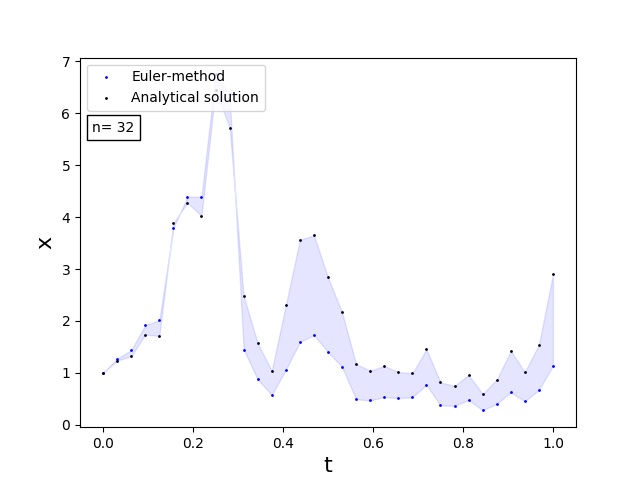
\includegraphics[scale=0.4]{Content/Graphics/SDE_EulerGBM_n_32}
   \end{subfigure}
   \begin{subfigure}{0.49\linewidth} \centering
     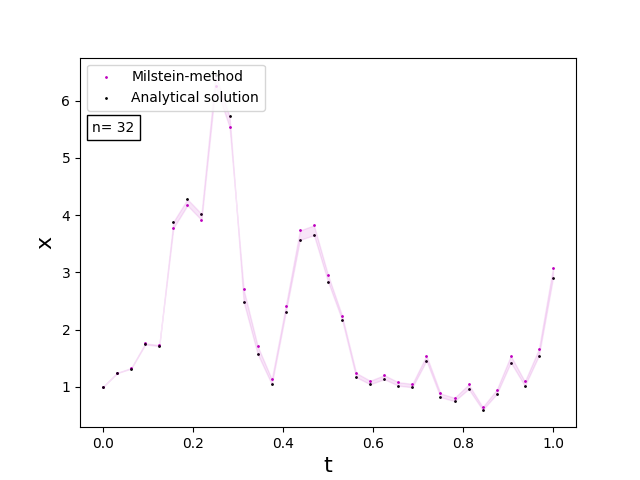
\includegraphics[scale=0.4]{Content/Graphics/SDE_MilsteinGBM_n_32}
   \end{subfigure}
   \begin{subfigure}{0.49\linewidth} \centering
     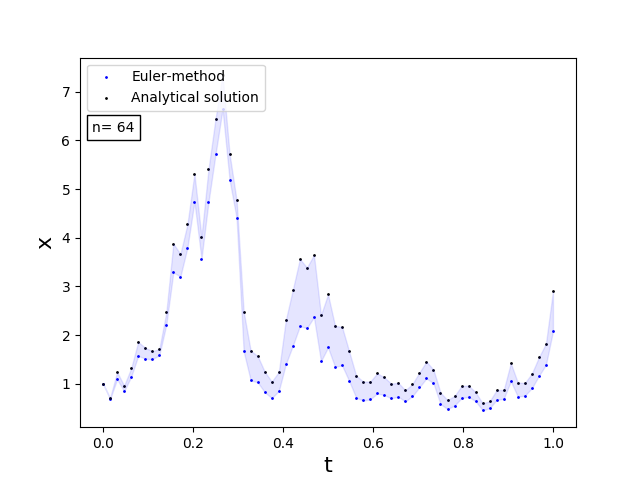
\includegraphics[scale=0.4]{Content/Graphics/SDE_EulerGBM_n_64}
   \end{subfigure}
   \begin{subfigure}{0.49\linewidth} \centering
     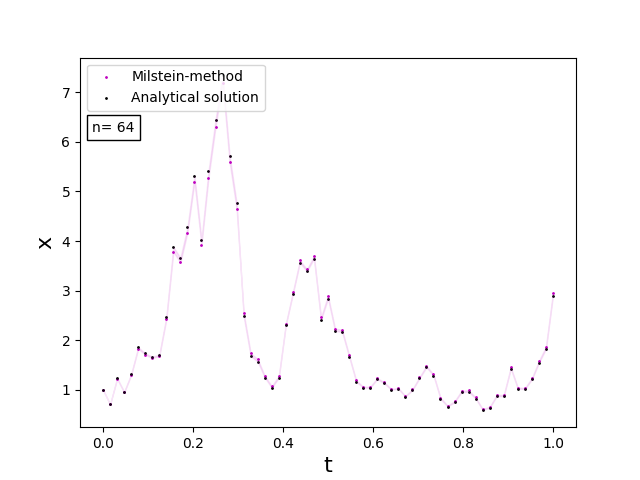
\includegraphics[scale=0.4]{Content/Graphics/SDE_MilsteinGBM_n_64}
   \end{subfigure}
\caption{Approximation (colored dots) of the sample path of the geometric Brownian motion and the true sample path (black dots) for n = 32, 64.}
\end{figure}


We did the same analysis for the Ornstein-Uhlenbeck process. Note that this process has a constant diffusion term (\(b(x)=\sigma\)). Thus the additional term of the Milstein-schem vanishes and the Euler- and the Milstein-scheme give the same results. Indeed the error-bound of the Milstein-scheme also applies to the Euler-Scheme for stochastic differential equations with constant diffusion terms. The Euler-scheme has convergence order 1.0 in this particular case.
In the following figures we can see that both schemes yield the same result:
\vfill
\begin{figure}[!h]
\centering
   \begin{subfigure}{0.49\linewidth} \centering
     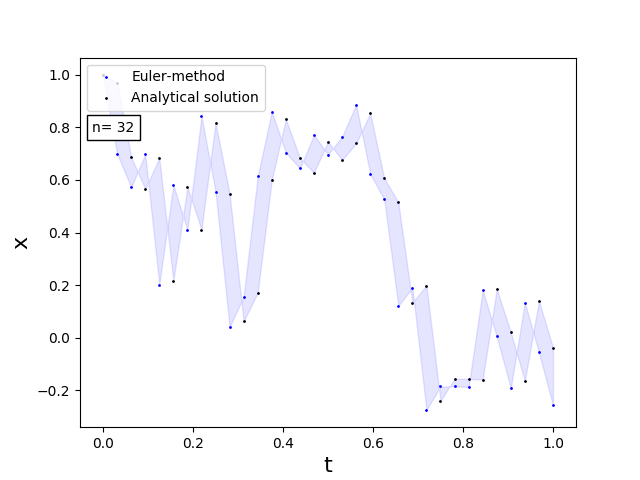
\includegraphics[scale=0.4]{Content/Graphics/SDE_EulerOU_n_32}
   \end{subfigure}
   \begin{subfigure}{0.49\linewidth} \centering
     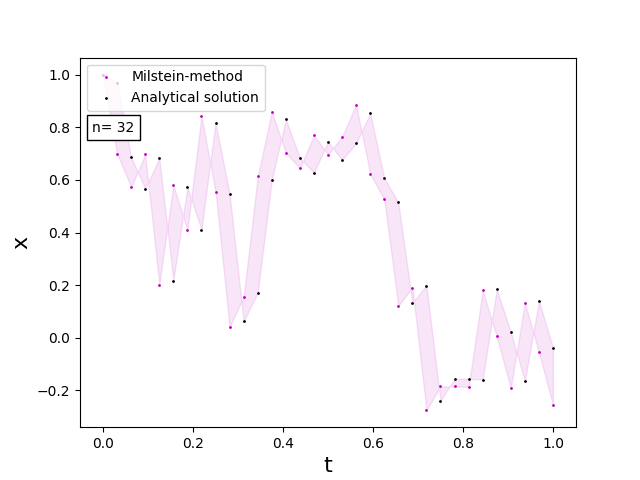
\includegraphics[scale=0.4]{Content/Graphics/SDE_MilsteinOU_n_32}
   \end{subfigure}
   \begin{subfigure}{0.49\linewidth} \centering
     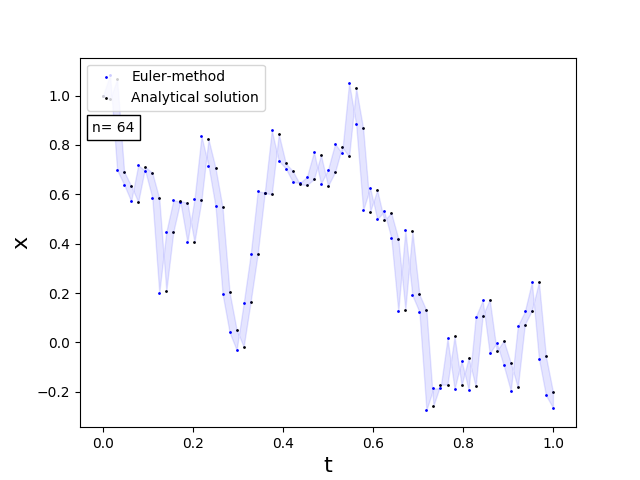
\includegraphics[scale=0.4]{Content/Graphics/SDE_EulerOU_n_64}
   \end{subfigure}
   \begin{subfigure}{0.49\linewidth} \centering
     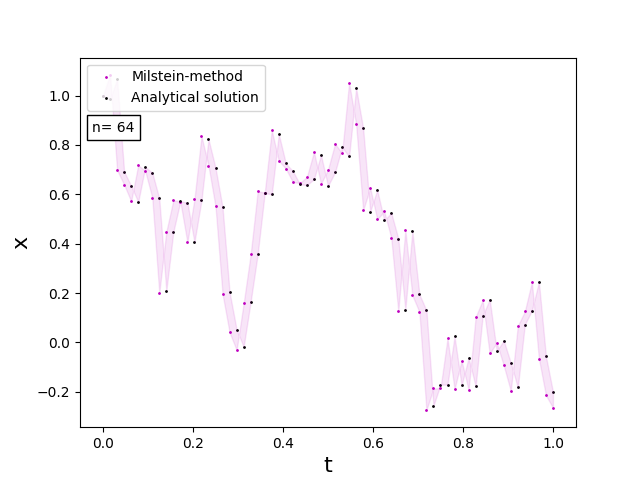
\includegraphics[scale=0.4]{Content/Graphics/SDE_MilsteinOU_n_64}
   \end{subfigure}
\caption{Approximation (colored dots) of the sample path of the Ornstein-Uhlenbeck process and the true sample path (black dots) for n = 32, 64.} 
\end{figure}


The next figures (figure \ref{fig:erroranalysis}) verify that the approximation error \(e_n\) is tending to 0 for increasing step amount n for both, the geometric Brownian motion and the Ornstein-Uhlenbeck process.\\
The approximation errors \(e_n\) have been calculated for \(n = 2^3,\ldots, 2^{10}\). Recall:
\[e_n\coloneqq\mathbb{E}[(X_T - \overline{X}^{n}_{T})^2]^{\frac{1}{2}}.\]

We then took the Monte-Carlo estimates using m = 100'000 simulations for each n. The estimate \(\hat{e}_n\) is defined as follows:
\[\hat{e}_n\coloneqq (\frac{1}{m}\sum_{k=1}^{m}(X_T^k - \overline{X}^{n,k}_{T})^2)^{\frac{1}{2}}\]
for given sample paths \(X_t^1,\ldots, X_t^m\) and the corresponding approximations \(\overline{X}^{n,1}_{t},\ldots,\overline{X}^{n,m}_{t}\).
We did this analysis using the Euler- and the Milstein-scheme and for each step amount n which we set previously.
\begin{figure}[!h]

\centering
   \begin{subfigure}{0.49\linewidth} \centering
     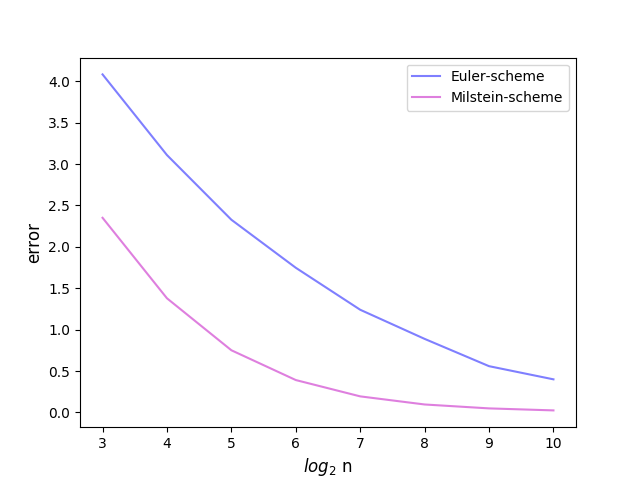
\includegraphics[scale=0.4]{Content/Graphics/ConvergenceEulerMilsteinGBM}
   \end{subfigure}
   \begin{subfigure}{0.49\linewidth} \centering
     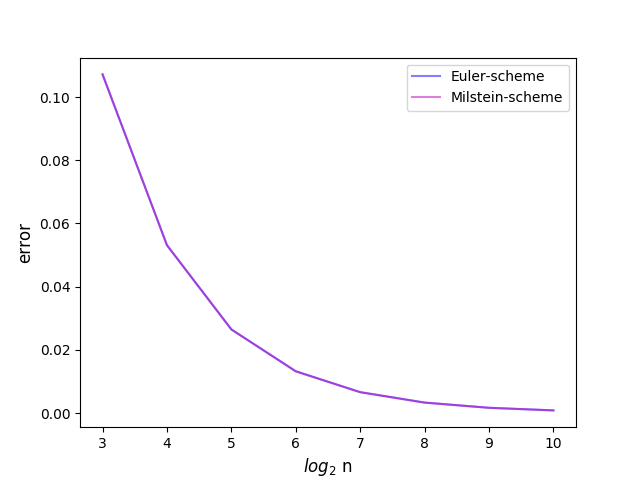
\includegraphics[scale=0.4]{Content/Graphics/ConvergenceEulerMilsteinOU}
   \end{subfigure}
\caption{Monte-Carlo estimates of the approximation error and the step amount n (logarithmized) for the geometric Brownian motion (left) and the Ornstein-Uhlenbeck process (right).} 
\label{fig:erroranalysis}
\end{figure}

The final figures (figure \ref{fig:convergenceanalysis}) show the log-log plot for the estimates of the approximation error and the step amount n. As was discussed in section \ref{erroranalysis} the (absolute value) of the slope of the regression line is an estimate for the convergence order.
The estimated convergence orders for the geometric Brownian motion match the analytical results. (0.5 for the Euler-scheme and 1.0 for the Milstein-Scheme). The same analysis on the Ornstein-Uhlenbeck process yields an order of 1.0 for both schemes.
However this is always the case if the diffusion term of the stochastic differential equation is constant, as we discussed previously. 
Our estimates for the convergence orders are:
\begin{enumerate}[noitemsep,topsep=0mm,labelindent=6mm,leftmargin=*,widest=3.,align=right]
\item Geometric Brownian motion:
\begin{enumerate}[noitemsep,topsep=0mm,labelindent=6mm,leftmargin=*,widest=3.,align=right]
\item Euler: 0.482.
\item Milstein: 0.950. 
\end{enumerate}
\item Ornstein-Uhlenbeck process:
\begin{enumerate}[noitemsep,topsep=0mm,labelindent=6mm,leftmargin=*,widest=3.,align=right]
\item Euler: 1.003.
\item Milstein: 1.003.
\end{enumerate}
\end{enumerate}

\begin{figure}[!h]

\centering
   \begin{subfigure}{0.49\linewidth} \centering
     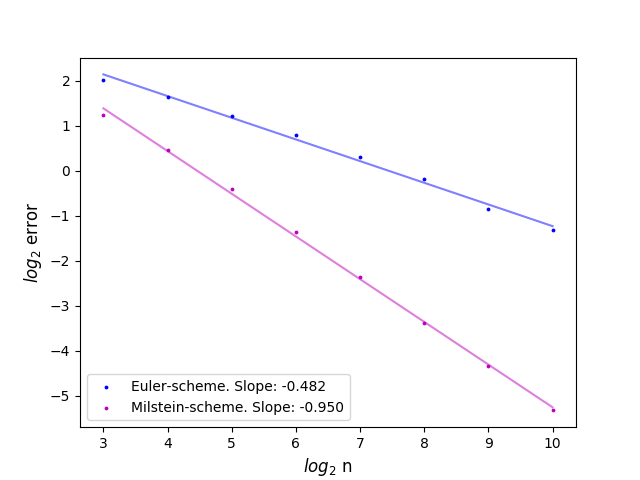
\includegraphics[scale=0.4]{Content/Graphics/Convergence_OrderEulerMilsteinGBM}
   \end{subfigure}
   \begin{subfigure}{0.49\linewidth} \centering
     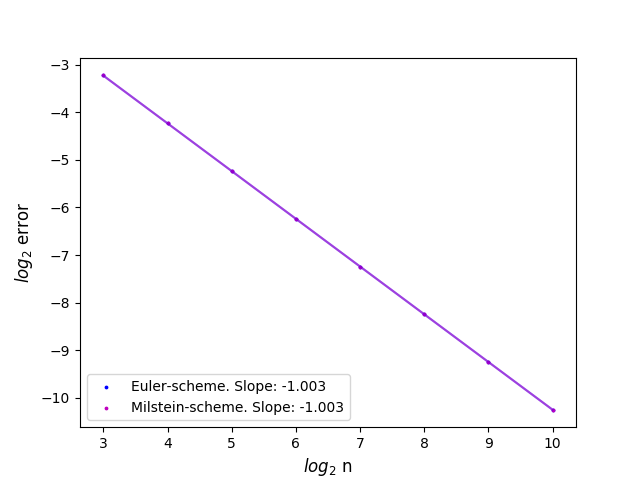
\includegraphics[scale=0.4]{Content/Graphics/Convergence_OrderEulerMilsteinOU}
   \end{subfigure}
\caption{Log-log plot of the approximation error and the step amount n for the geometric Brownian motion (left) and the Ornstein-Uhlenbeck process (right).} 
\label{fig:convergenceanalysis}
\end{figure}
\vfill

\section{Conclusion}

We conclude that even for a low amount of discretization steps n, the Milstein-scheme gives an impressive approximation for the true sample paths. The implementation is not difficult and should always be prefered over the Euler-scheme.
More graphics can be seen in appendix \ref{Graphics}. We also verified the (theoretical) convergence orders numerically.\\

However we remark that the conditions for both schemes (globally Lipschitz) are quite strong and therefore the schemes do not allow for coefficients which do not fulfill these conditions. There are many stochastic differential equations which have non-Lipschitz coefficients. Further research can be done by finding the convergence proofs which works for weaker conditions. Better (in terms of higher convergence order) schemes, if necessary, can be obtained by iteratively applying the It\^o-lemma on the coefficients and by truncating these stochastic Taylor expansions (given that the coefficients are smooth enough). However these higher-order schemes become complex very quickly.\\

One might think that there is also a generalization of the Heun-method for stochastic differential equations, since also the Euler-Maruyama method is a generalization of a well-known method from deterministic analysis. The Heun-method is based on the trapezoid-rule from numerical integration theory. Since we are operating with It\^o stochastic integrals, we cannot apply the trapezoid rule (recall the definition of the It\^o stochastic integral). However there exist implicit schemes and also derivative-free schemes (Runge-Kutta) for stochastic differential equations and we refer to \cite{KloedenPlaten} for their treatment.\\

We end the thesis with the final remark that numerical schemes for stochastic differential equations are obtained in a similair way as their deterministic counterparts. We also used methods which are analogous to the Taylor expansion in order to construct our approximation schemes, by truncating these expansions. However we cannot blindly generalize methods from (deterministic) numerical analysis. We do need to take the stochastic setting into our consideration. In our case, this was the It\^o stochastic calculus.
Therefore it is inevitable to have profound knowledge in stochastic analysis, if one wishes to construct numerical schemes for stochastic differential equations.













\appendix
%\chapter{Proof: Existence and uniqueness of solutions}
%\label{Proof:ExistenceUniqueness}




\chapter{Gronwall-inequality}
\label{Gronwall}
\begin{lemma}[Gronwall-inequality]
Let \(\phi\) and f be nonnegative and continuous functions defined on [0,T]. Let $C>0$ denote a constant. If:
\[\phi(t)\leq C + \int_0^t \! f(s)\phi(s)\,\mathrm{d}s\quad\text{for all}\:\:t\in[0,T]\]
then:
\[\phi(t)\leq C\cdot\exp(\int_0^t \! f(s)\,\mathrm{d}s) \quad\text{for all}\:\:t\in[0,T].\]
\end{lemma}
\begin{proof}

Let \(\psi(t)\) be defined as:
\[
\psi(t) = C + \int_0^t \! f(s)\phi(s)\,\mathrm{d}s.
\]
Given that \(\phi(t) \leq \psi(t)\), we substitute \(\phi(t)\) with \(\psi(t)\) in the integral:
\[
\psi(t) = C + \int_0^t \! f(s)\phi(s)\,\mathrm{d}s \leq C + \int_0^t \! f(s)\psi(s)\,\mathrm{d}s.
\]
Next, consider the function \(g(t)\) defined by:
\[
g(t) = \exp\left(-\int_0^t \! f(s)\,\mathrm{d}s\right)\psi(t).
\]
We now differentiate \(g(t)\) with respect to \(t\):
\[
\frac{\mathrm{d}g(t)}{\mathrm{d}t} = \exp\left(-\int_0^t \! f(s)\,\mathrm{d}s\right)\left[f(t)\psi(t) - f(t)\psi(t) + \frac{\mathrm{d}\psi(t)}{\mathrm{d}t}\right] = \exp\left(-\int_0^t \! f(s)\,\mathrm{d}s\right)\frac{\mathrm{d}\psi(t)}{\mathrm{d}t}.
\]
Since:
\[
\frac{\mathrm{d}\psi(t)}{\mathrm{d}t} = f(t)\phi(t),
\]
we get:
\[
\frac{\mathrm{d}g(t)}{\mathrm{d}t} = \exp\left(-\int_0^t \! f(s)\,\mathrm{d}s\right)f(t)\phi(t).
\]
Integrating from \(0\) to \(t\), we have:
\[
g(t) = g(0) + \int_0^t \exp\left(-\int_0^s \! f(\tau)\,\mathrm{d}\tau\right)f(s)\phi(s)\,\mathrm{d}s.
\]
At \(t = 0\), \(g(0) = C\). Therefore:
\[
\psi(t) \leq C\exp\left(\int_0^t \! f(s)\,\mathrm{d}s\right).
\]
Finally, since \(\phi(t) \leq \psi(t)\), we obtain:
\[
\phi(t) \leq C\cdot\exp\left(\int_0^t \! f(s)\,\mathrm{d}s\right).
\]
This completes the proof.

\end{proof}

\chapter{Source code}
\label{code}
The numerical methods presented in this thesis were implemented using Python. Key libraries include \texttt{Matplotlib} for plots and \texttt{NumPy} for numerical computations.

The complete source code with additional documentation and examples is available on GitHub at: \href{https://github.com/AmrUmeri/NumericalSDE}{\texttt{https://github.com/AmrUmeri/NumericalSDE}}. The repository contains all the necessary files to replicate the results presented in this thesis and instructions on how to run the code.

 
%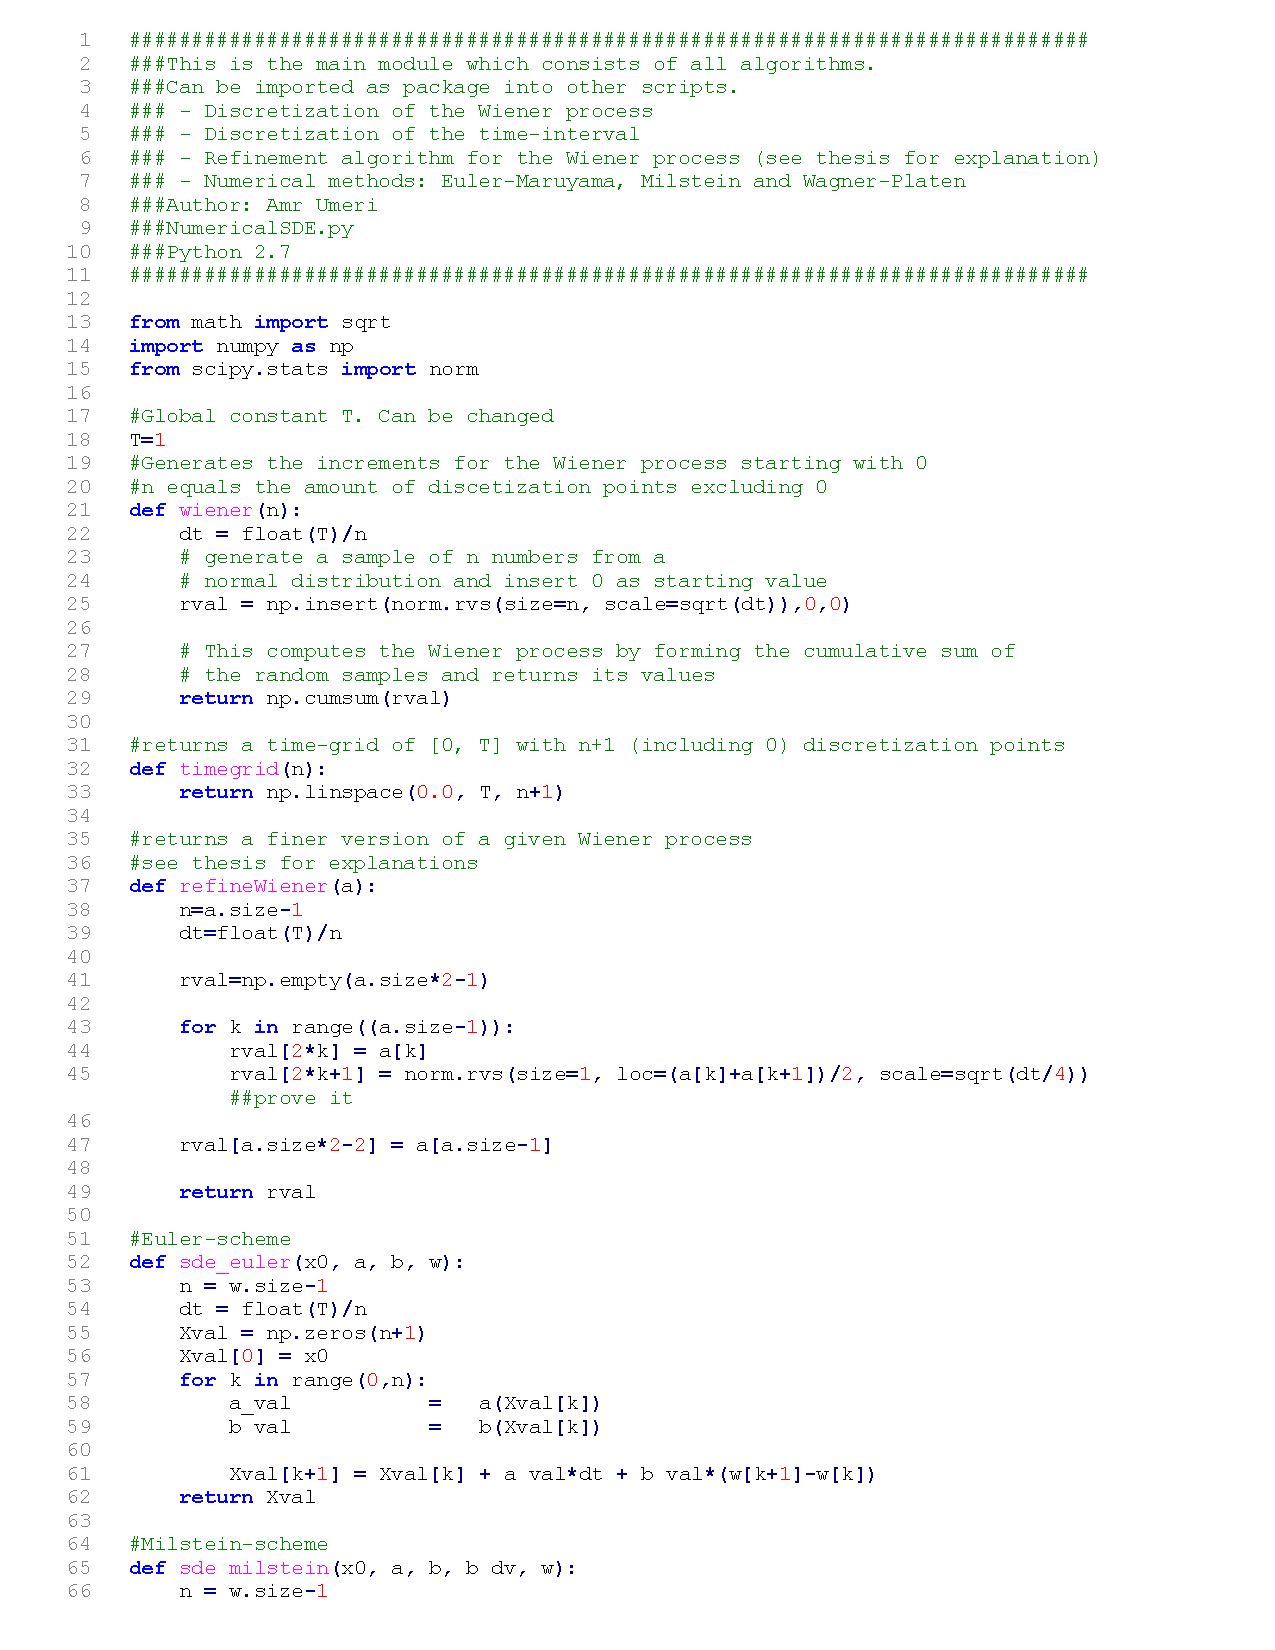
\includepdf[pages={-}]{Content/Code/NumericalSDE.pdf}
%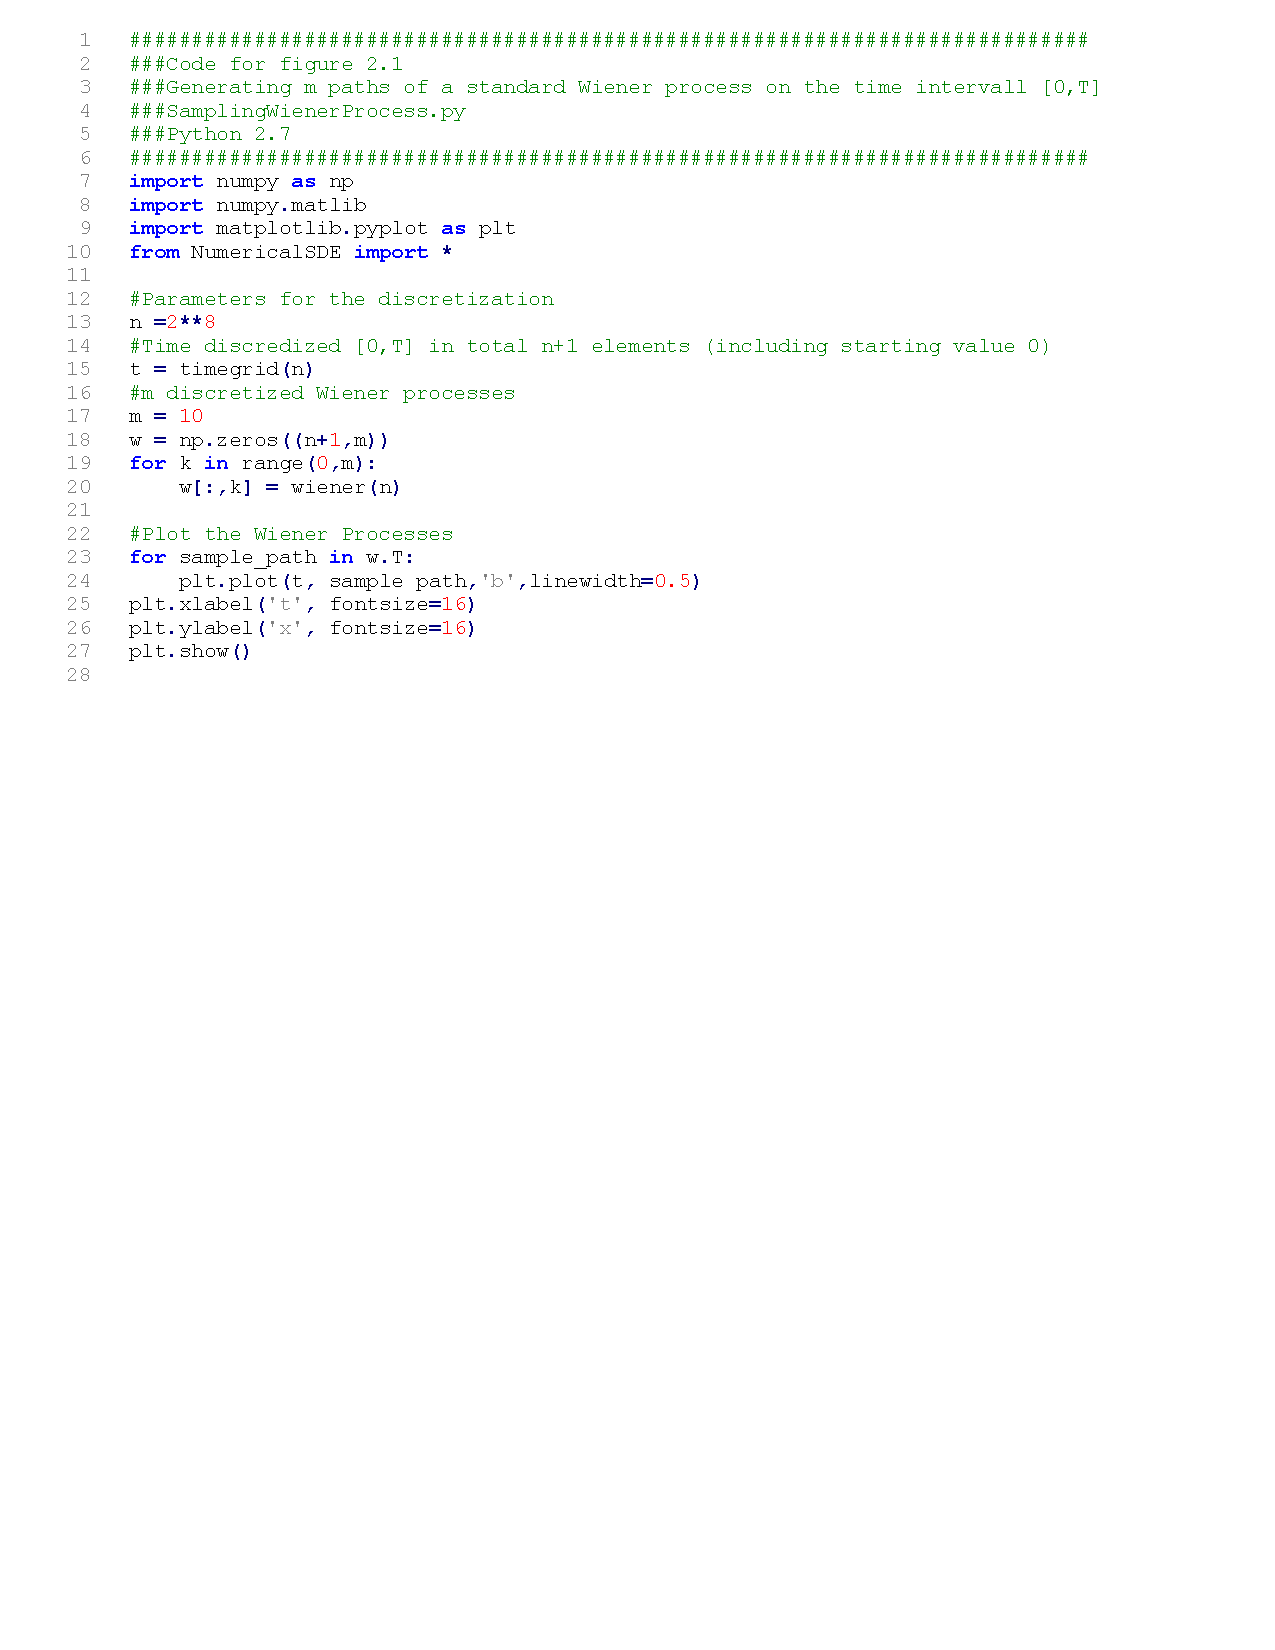
\includepdf[pages={-}]{Content/Code/SamplingWienerProcessGraphic.pdf}
%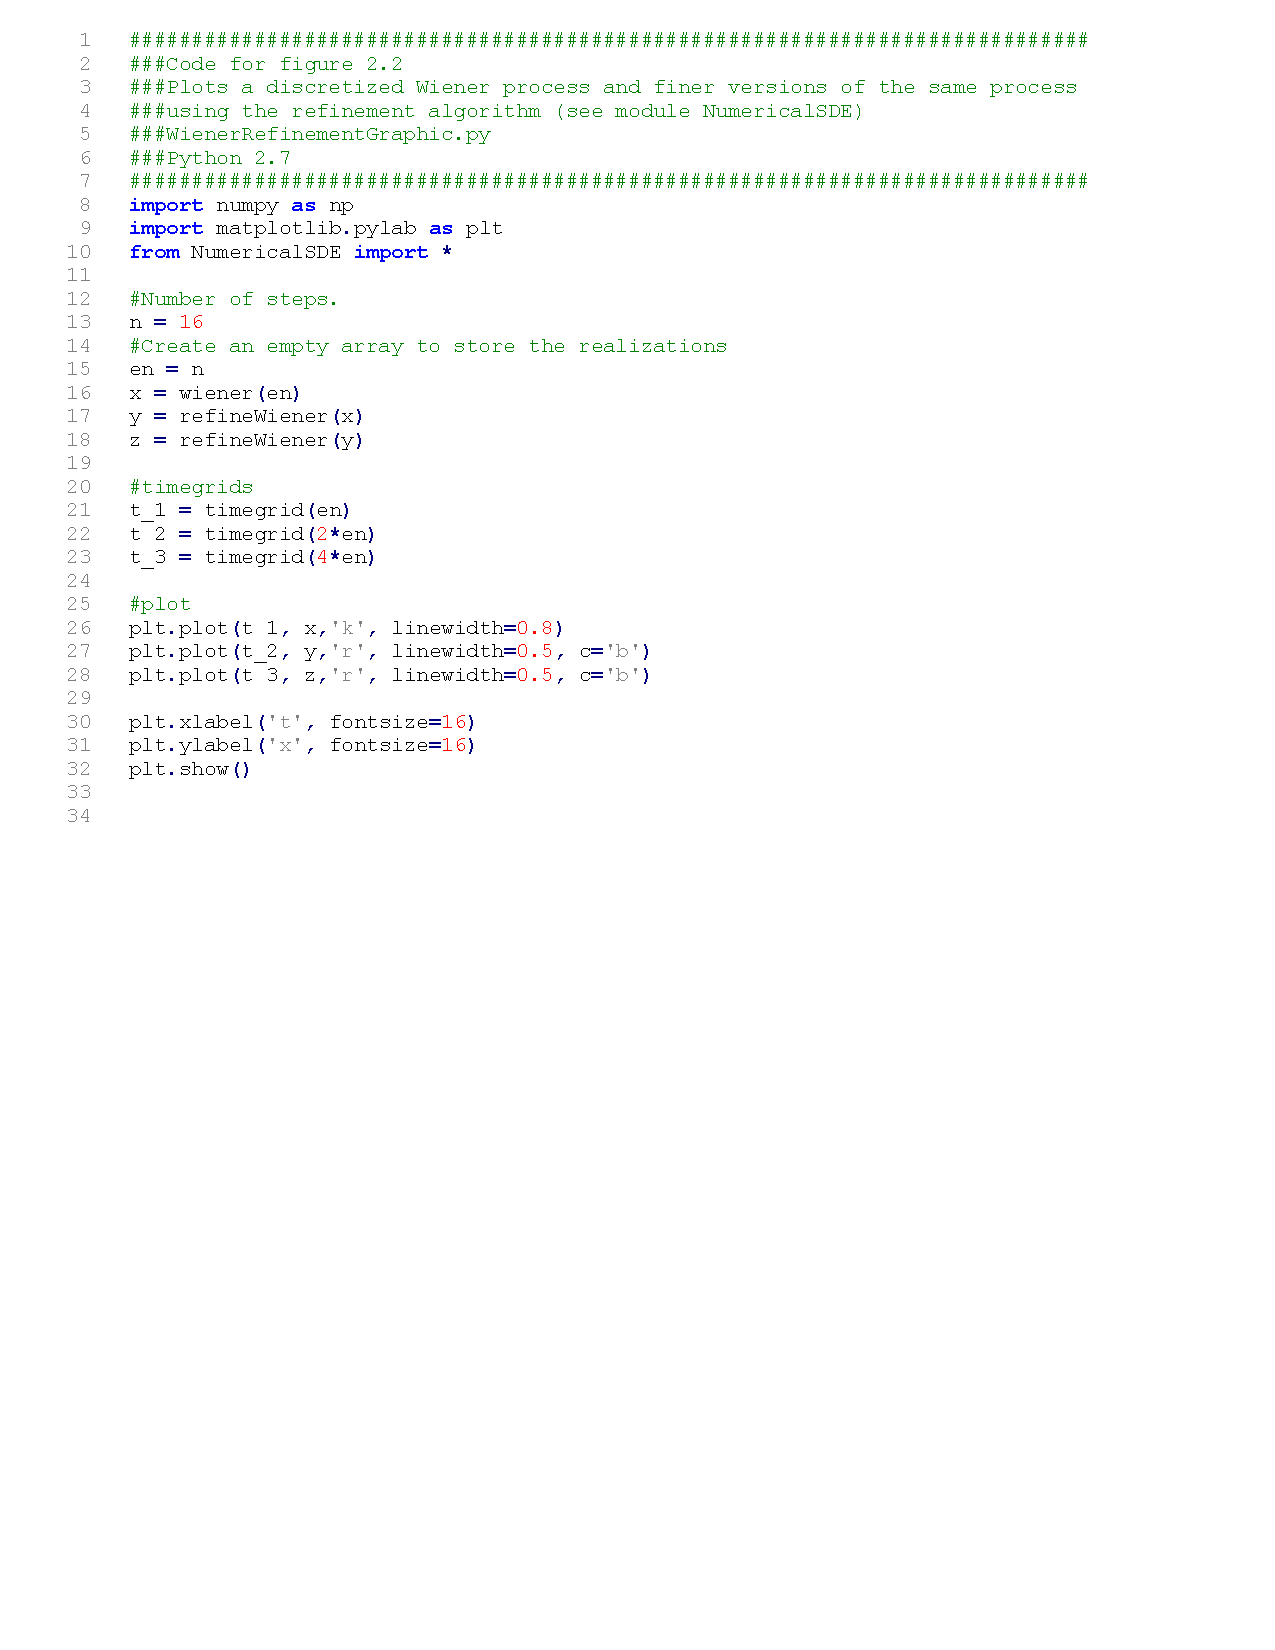
\includepdf[pages={-}]{Content/Code/WienerRefinementGraphic.pdf}
%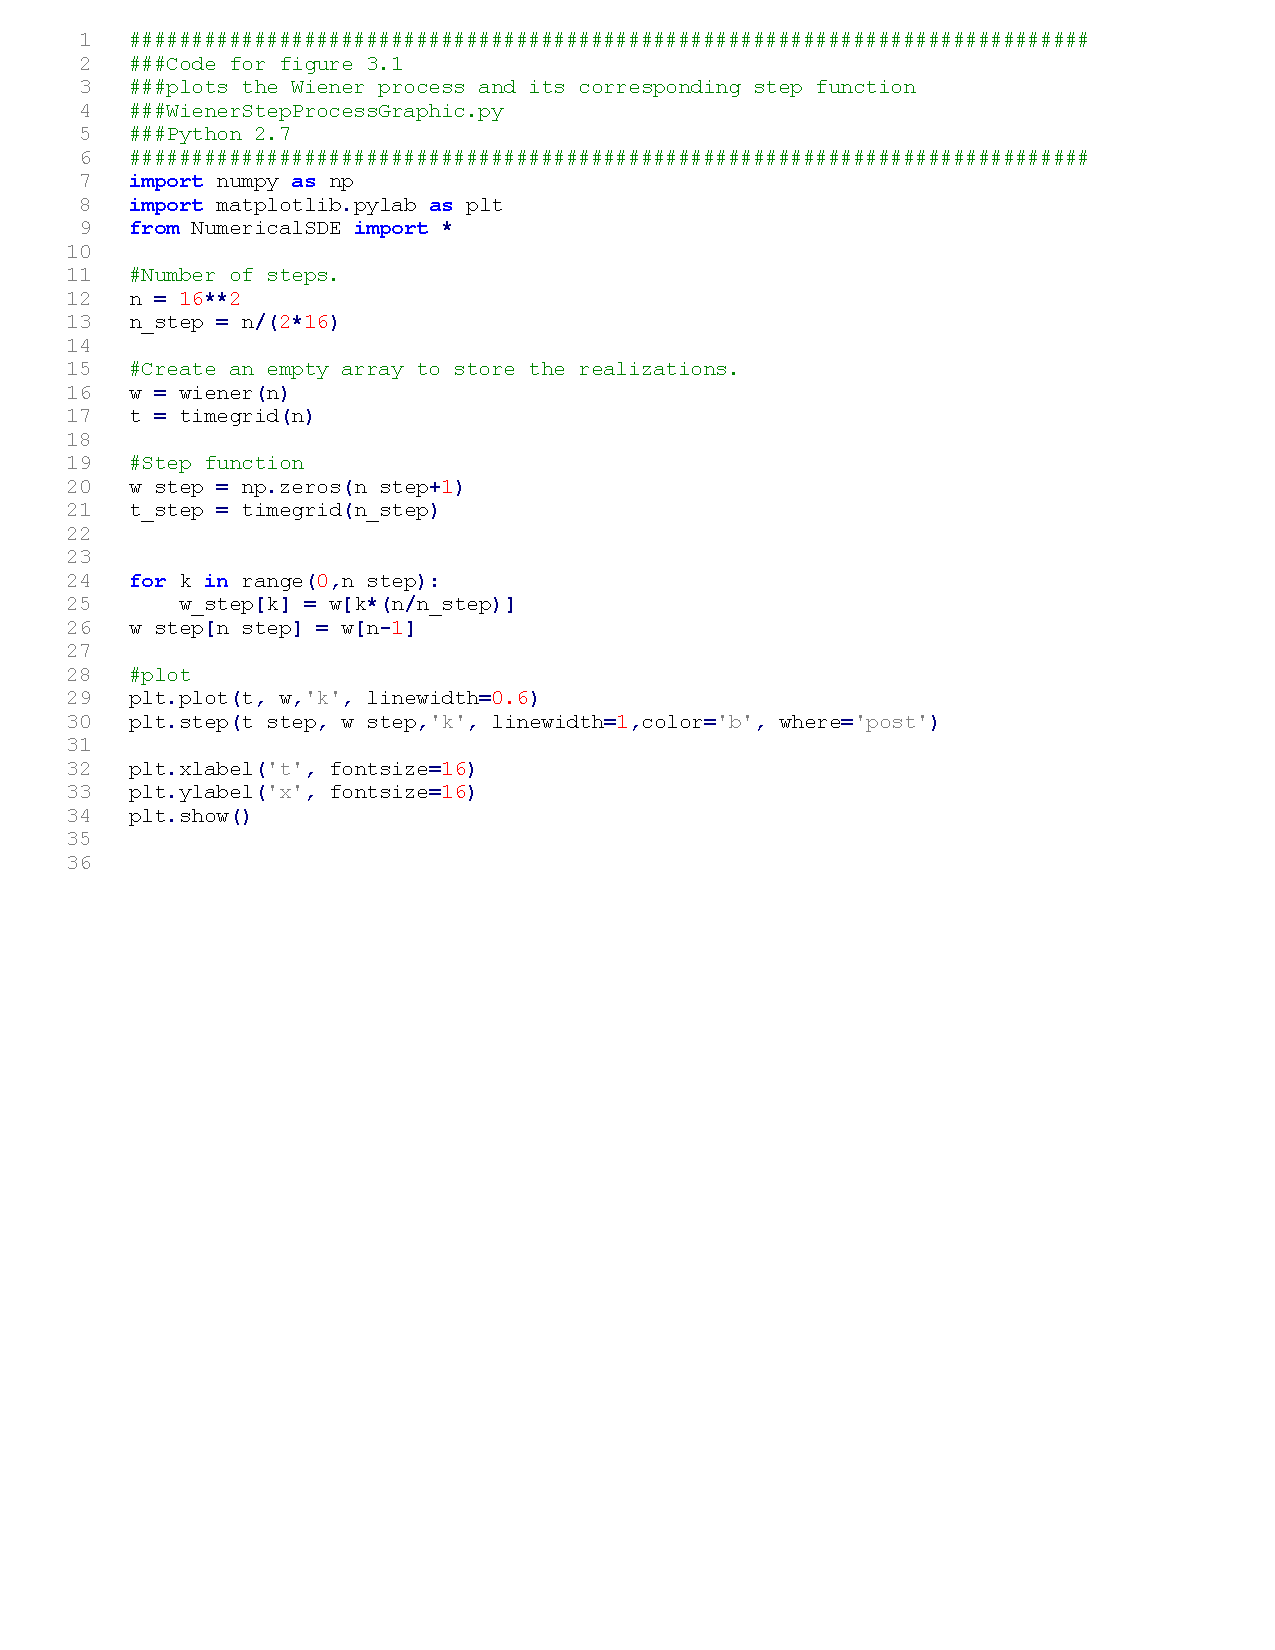
\includepdf[pages={-}]{Content/Code/WienerStepProcessGraphic.pdf}
%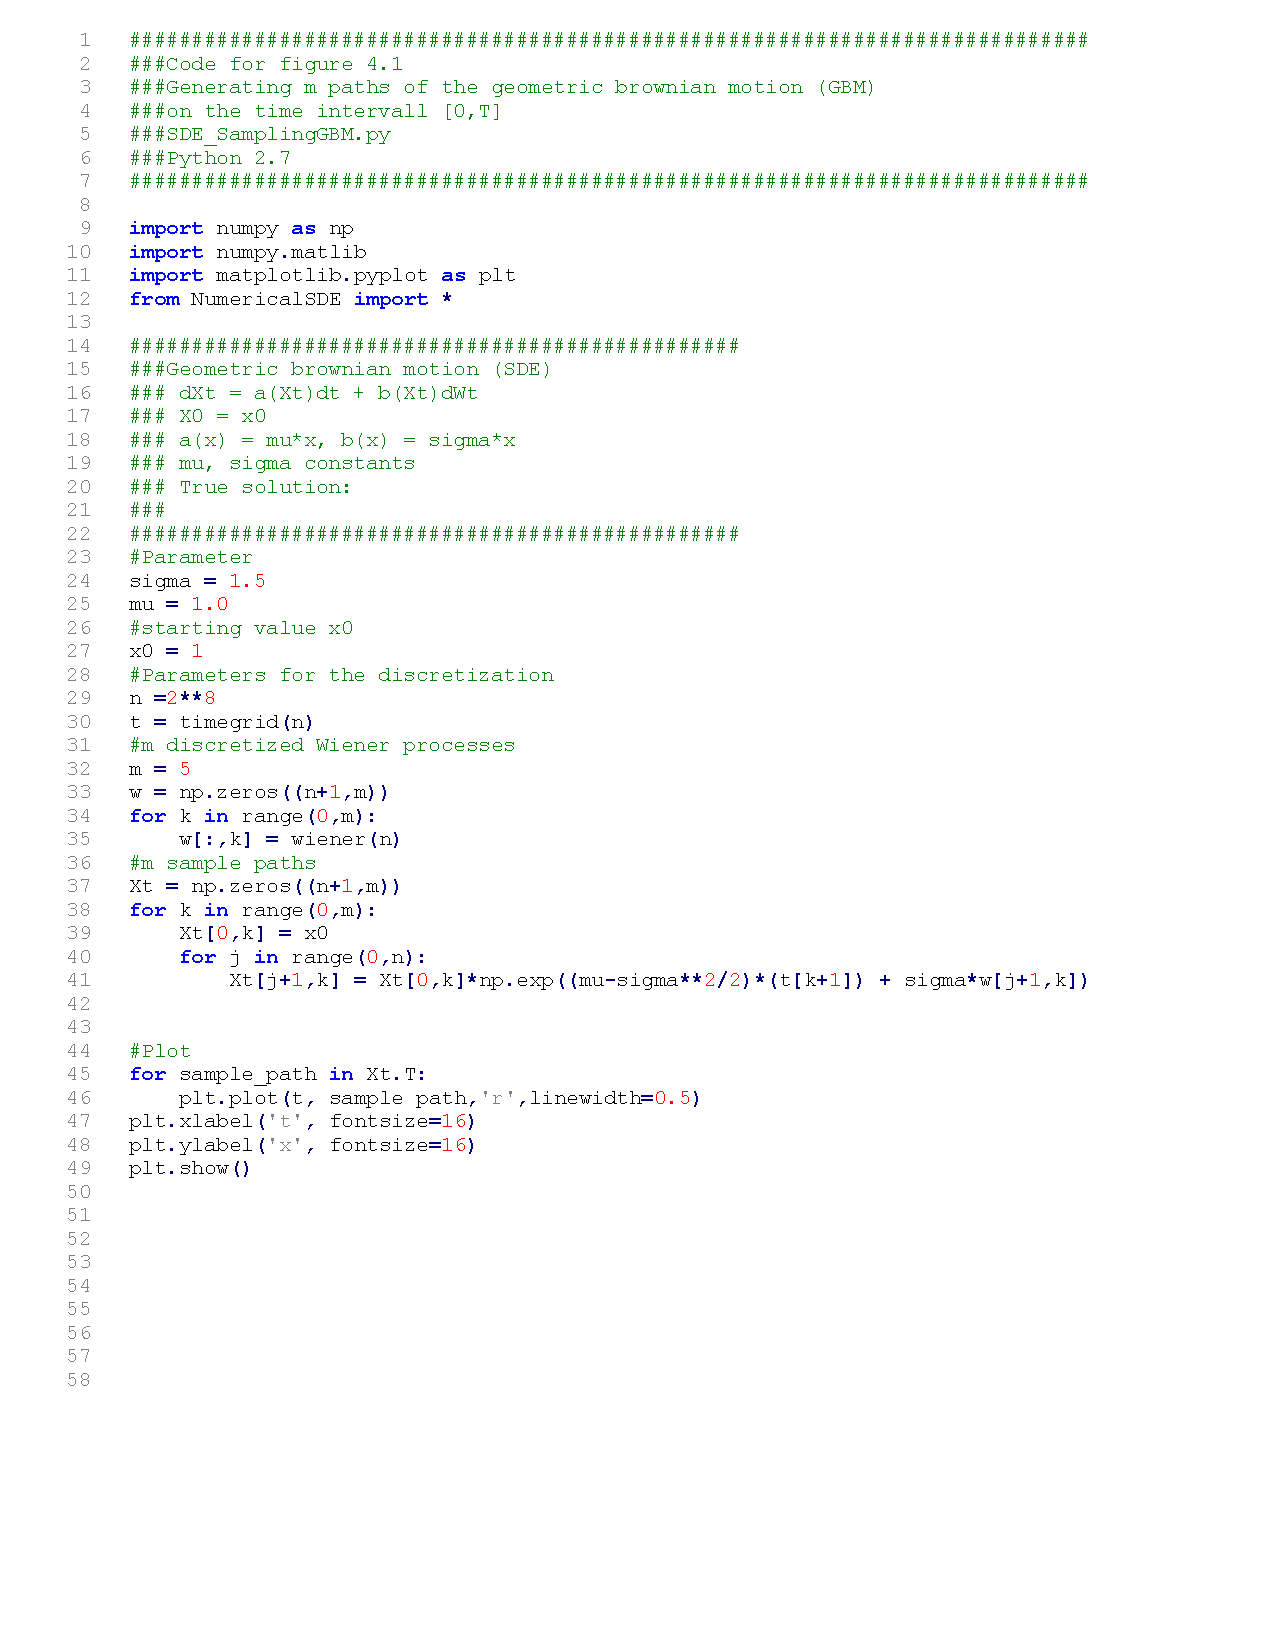
\includepdf[pages={-}]{Content/Code/SDE_SamplingGBM.pdf}
%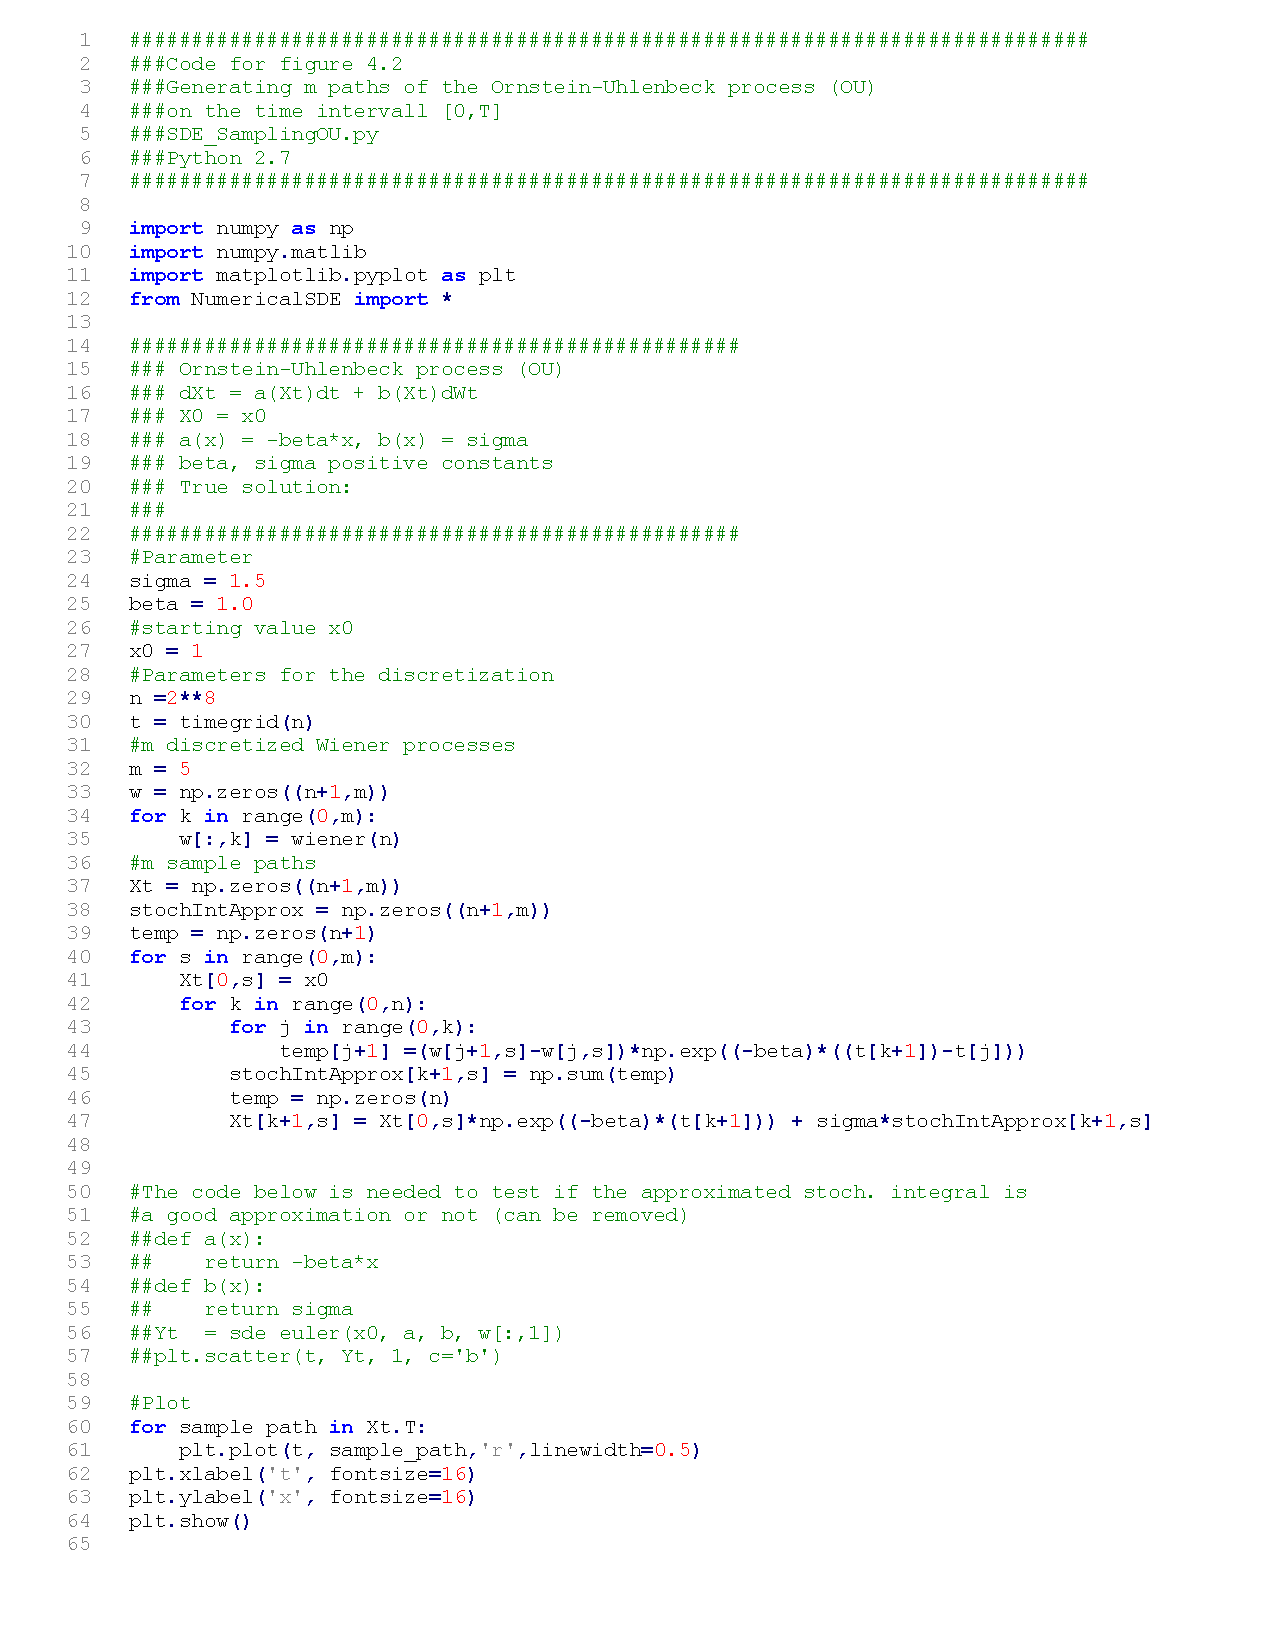
\includepdf[pages={-}]{Content/Code/SDE_SamplingOU.pdf}
%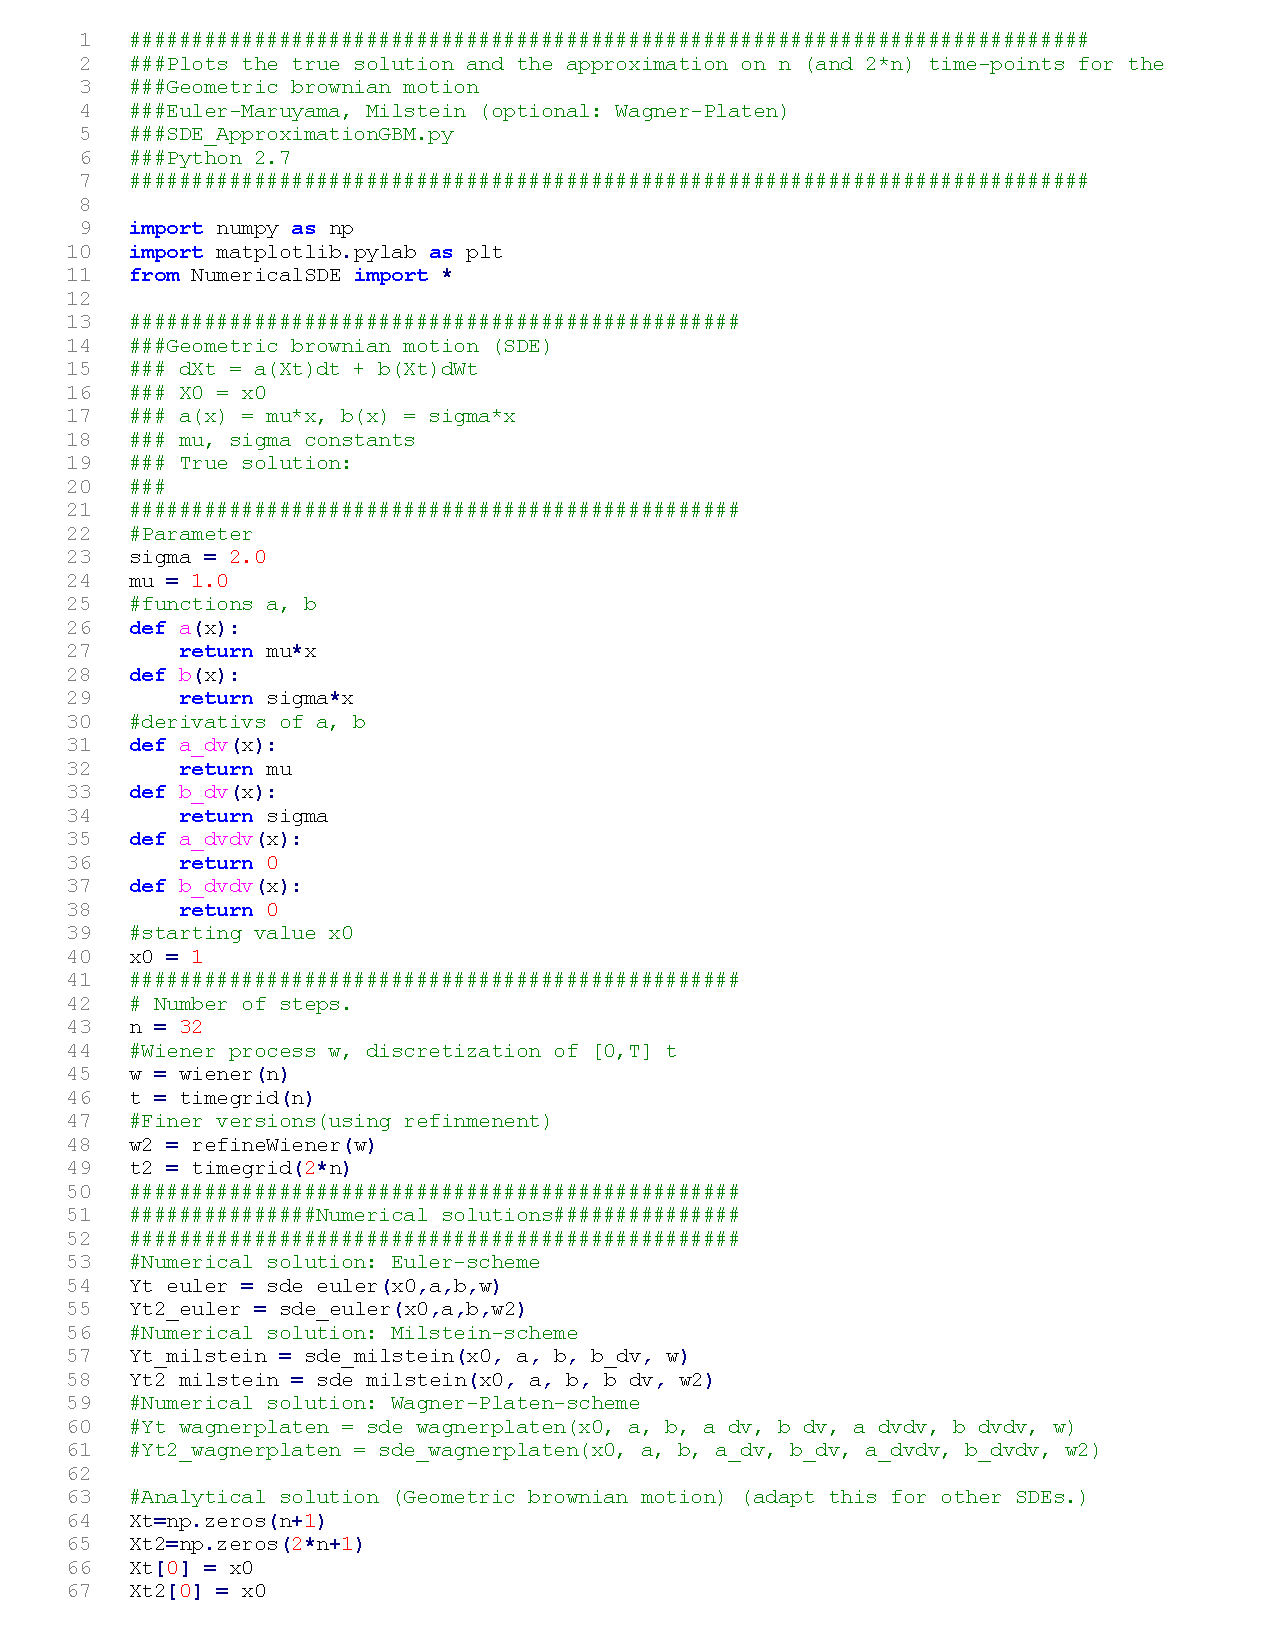
\includepdf[pages={-}]{Content/Code/SDE_ApproximationGBM.pdf}
%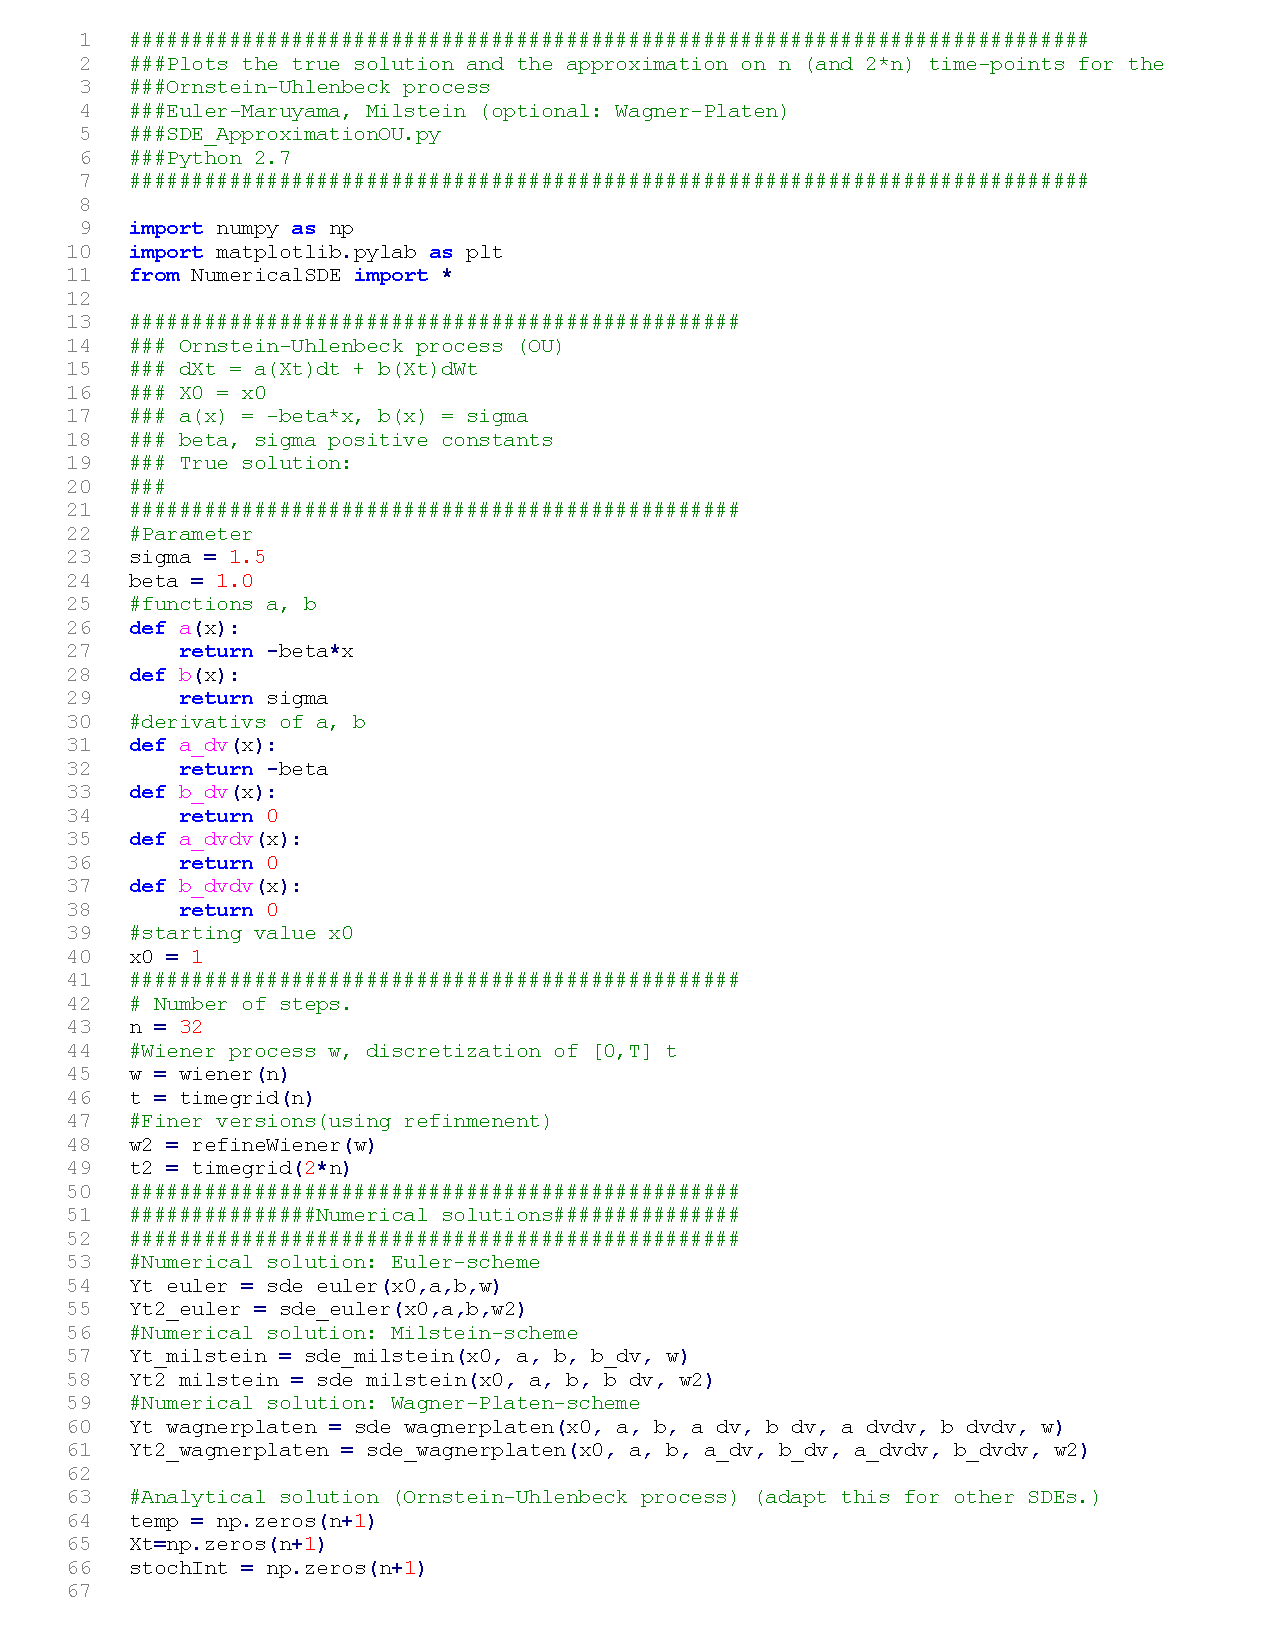
\includepdf[pages={-}]{Content/Code/SDE_ApproximationOU.pdf}
%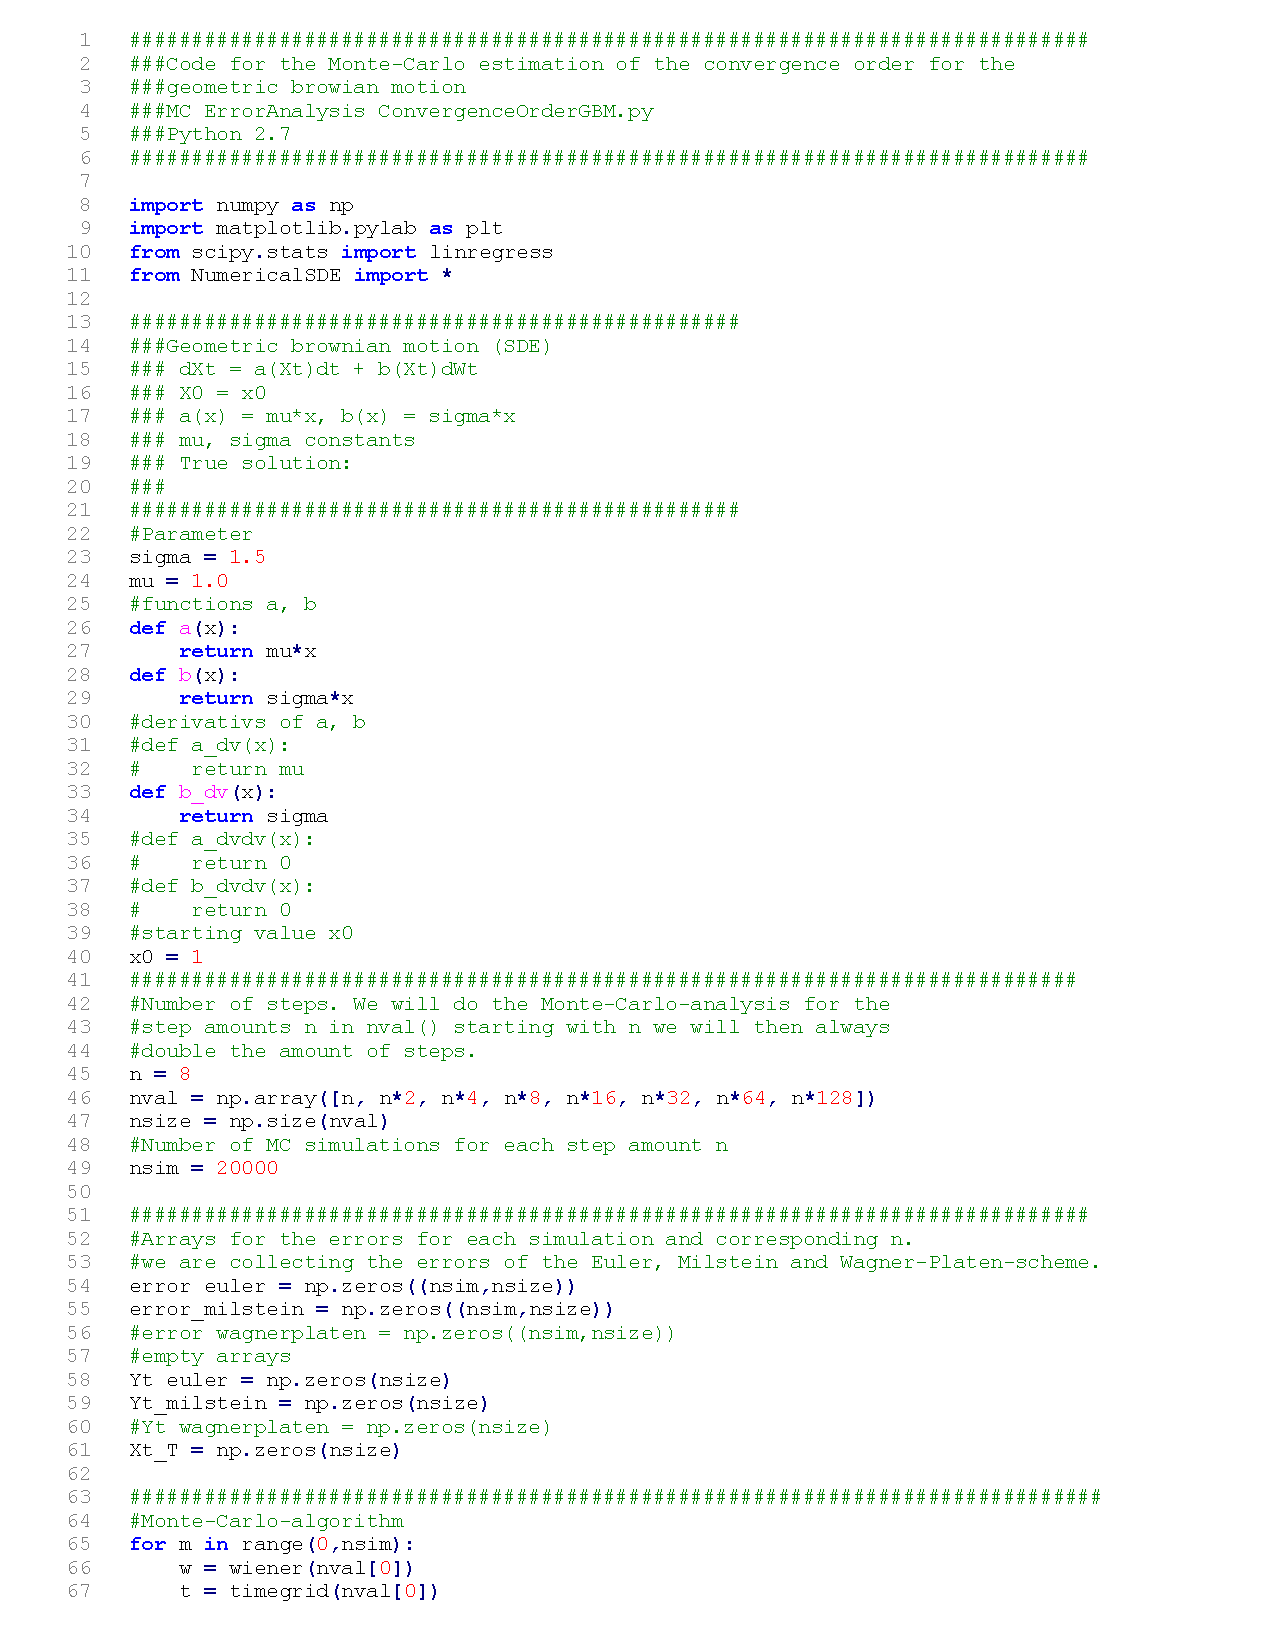
\includepdf[pages={-}]{Content/Code/MC_ConvergenceOrderGBM.pdf}
%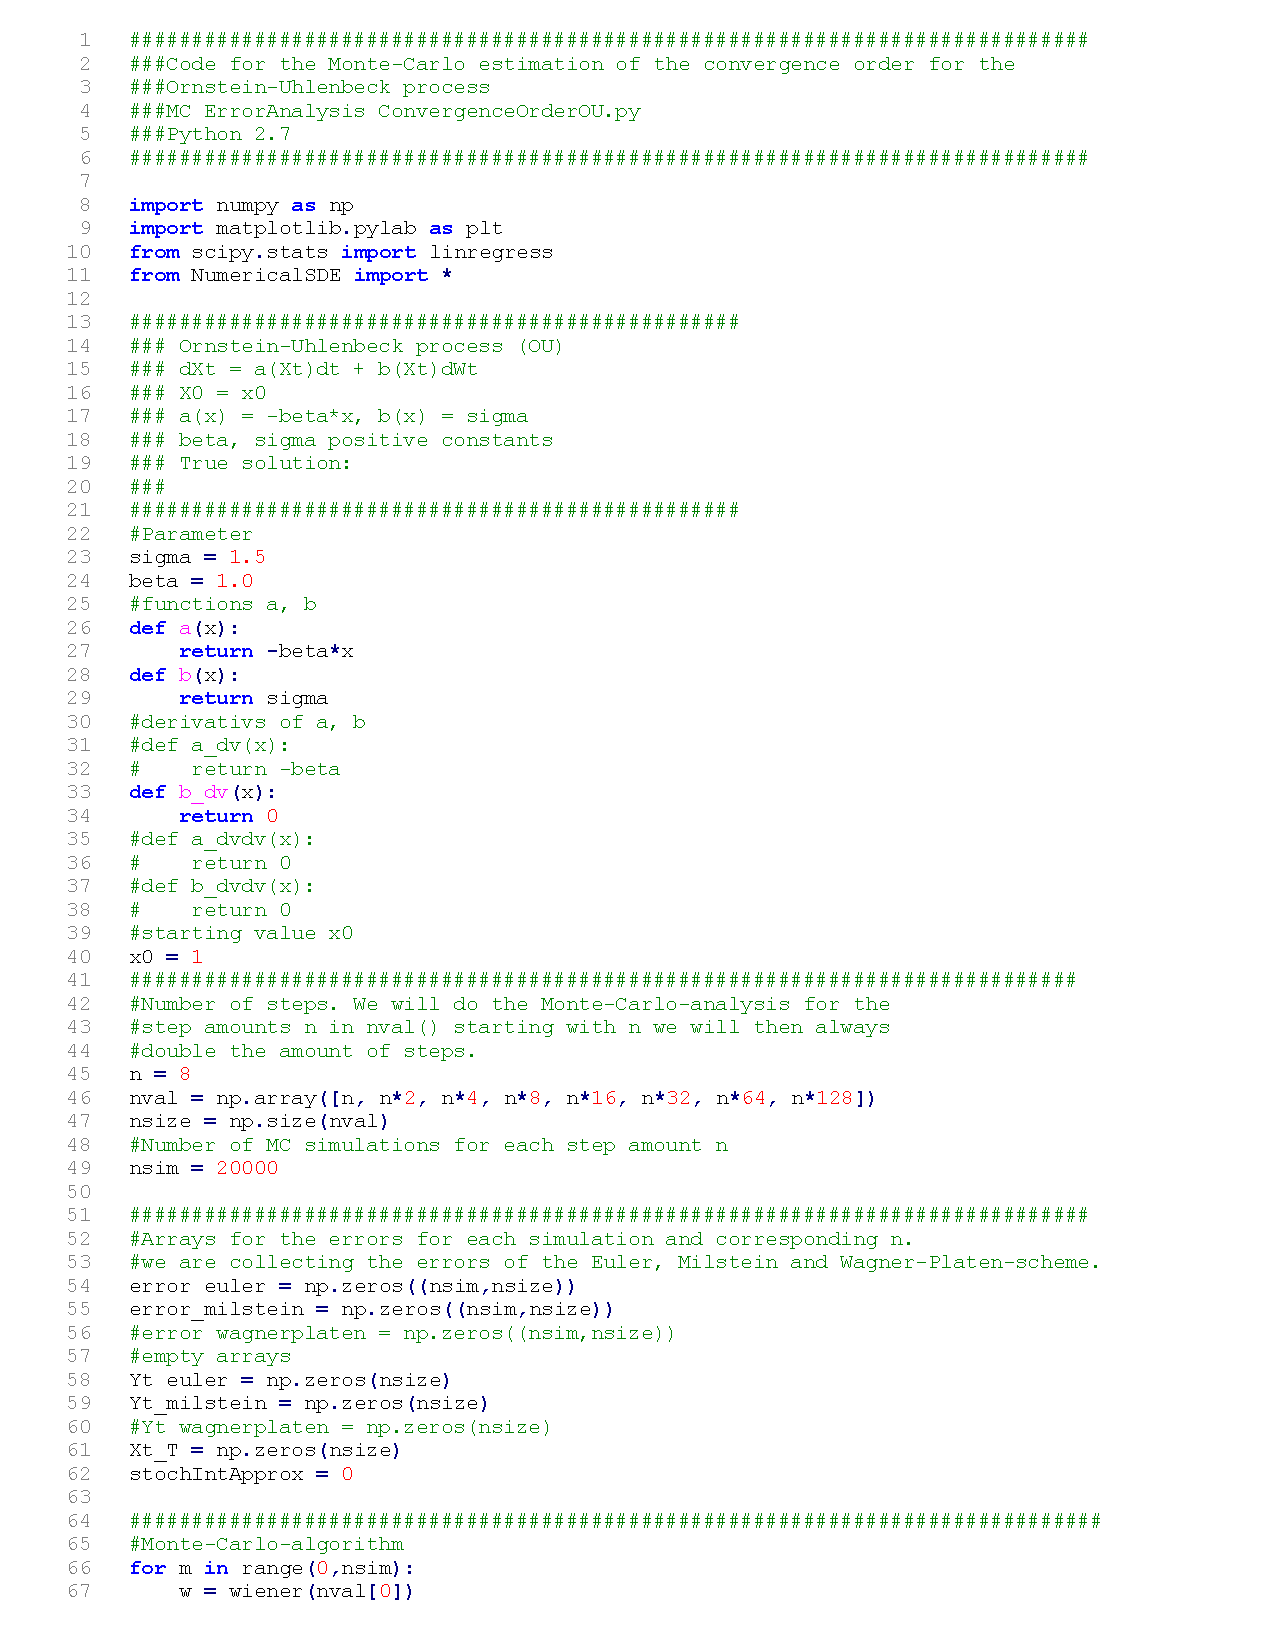
\includepdf[pages={-}]{Content/Code/MC_ConvergenceOrderOU.pdf}


\chapter{Additional plots}
\label{Graphics}
We included some additional figures in the next pages to illustrate the approximation schemes. Especially we also added some graphics of the Wagner-Platen approximation and its error-analysis. It has strong order 1.5. This scheme has not beed discussed in the main text of the thesis. However we implemented this scheme as well.


\begin{figure}[!h]
\centering
   \begin{subfigure}{0.49\linewidth} \centering
     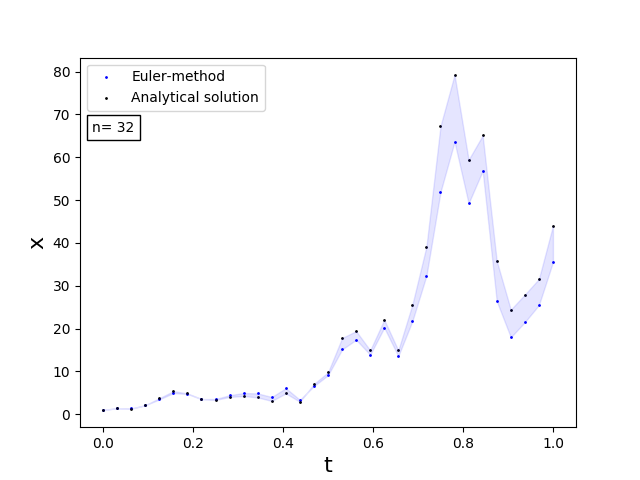
\includegraphics[scale=0.4]{Content/Graphics/Appendix/1gbm}
   \end{subfigure}
   \begin{subfigure}{0.49\linewidth} \centering
     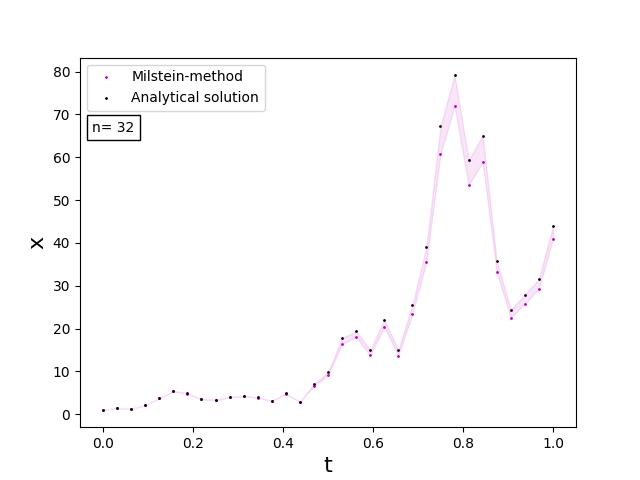
\includegraphics[scale=0.4]{Content/Graphics/Appendix/2gbm}
   \end{subfigure}
   \begin{subfigure}{0.49\linewidth} \centering
     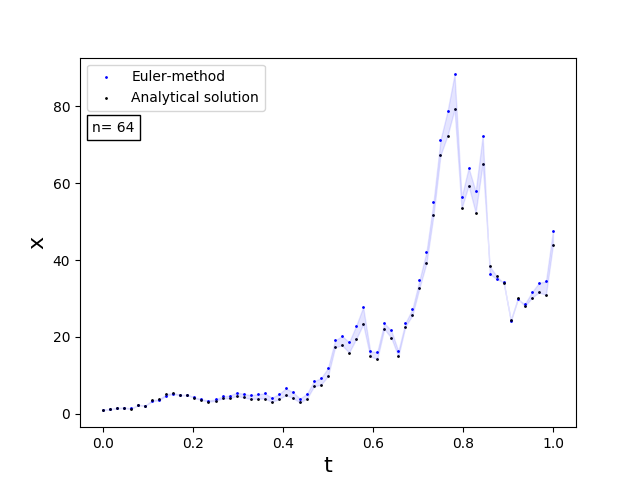
\includegraphics[scale=0.4]{Content/Graphics/Appendix/3gbm}
   \end{subfigure}
   \begin{subfigure}{0.49\linewidth} \centering
     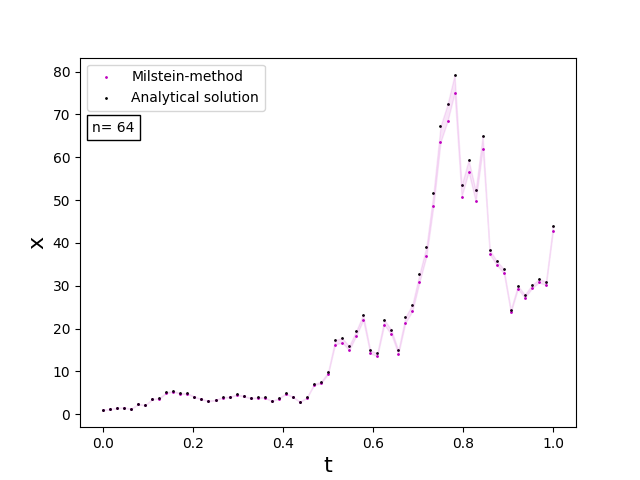
\includegraphics[scale=0.4]{Content/Graphics/Appendix/4gbm}
   \end{subfigure}
   \begin{subfigure}{0.49\linewidth} \centering
     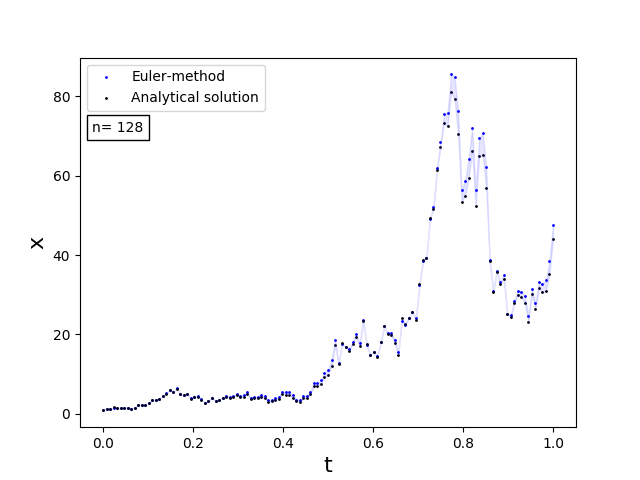
\includegraphics[scale=0.4]{Content/Graphics/Appendix/5gbm}
   \end{subfigure}
   \begin{subfigure}{0.49\linewidth} \centering
     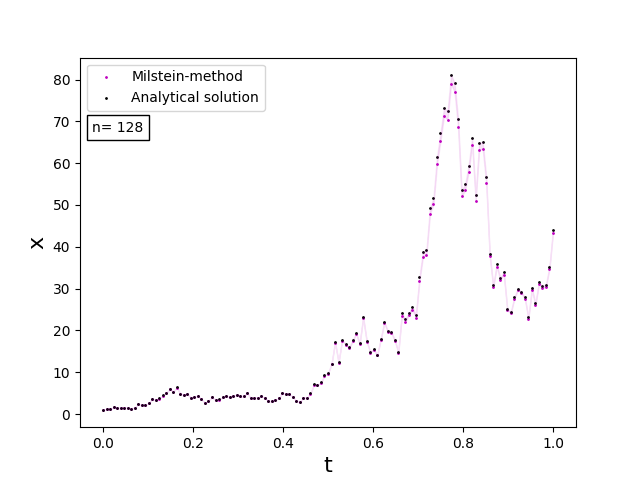
\includegraphics[scale=0.4]{Content/Graphics/Appendix/6gbm}
   \end{subfigure}
\caption{Approximation (colored dots) of the sample path of the geometric Brownian motion and the true sample path (black dots) for n = 32, 64, 128 using Euler and Milstein.}
\end{figure}

\begin{figure}[!h]
\centering
   \begin{subfigure}{0.49\linewidth} \centering
     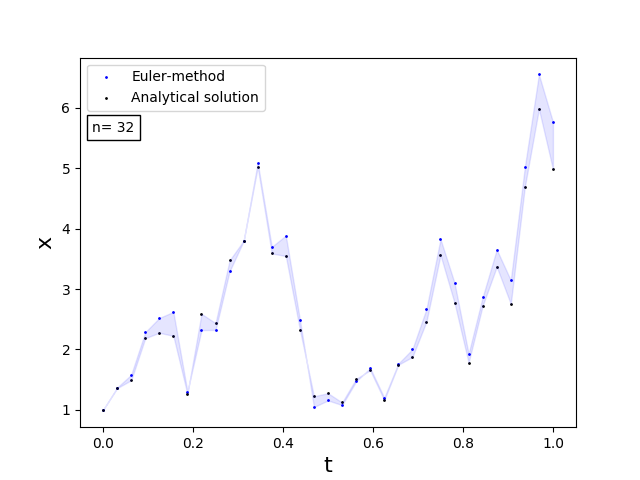
\includegraphics[scale=0.4]{Content/Graphics/Appendix/1gbm2}
   \end{subfigure}
   \begin{subfigure}{0.49\linewidth} \centering
     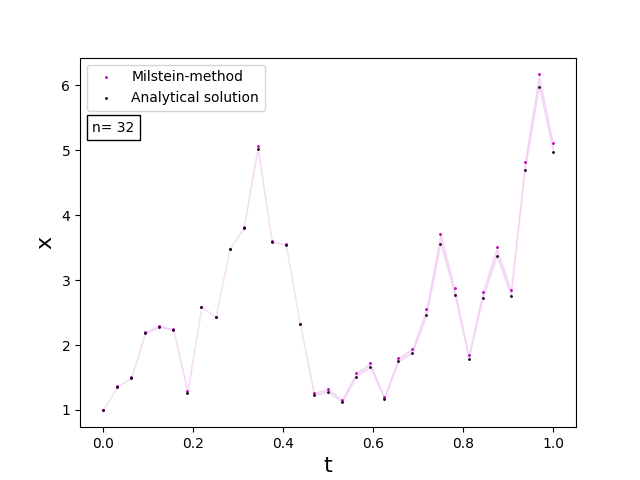
\includegraphics[scale=0.4]{Content/Graphics/Appendix/2gbm2}
   \end{subfigure}
   \begin{subfigure}{0.49\linewidth} \centering
     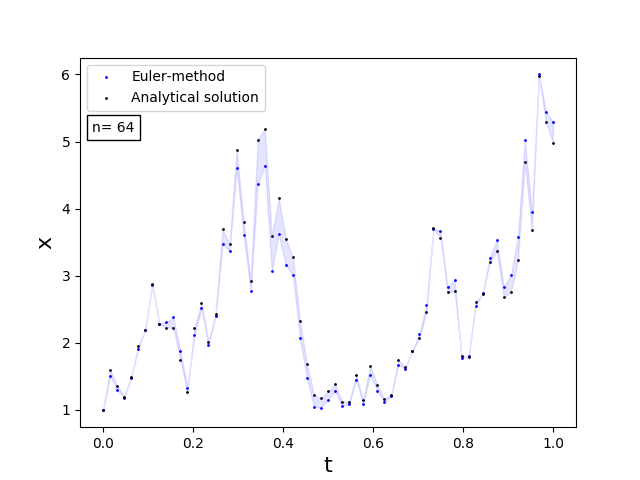
\includegraphics[scale=0.4]{Content/Graphics/Appendix/3gbm2}
   \end{subfigure}
   \begin{subfigure}{0.49\linewidth} \centering
     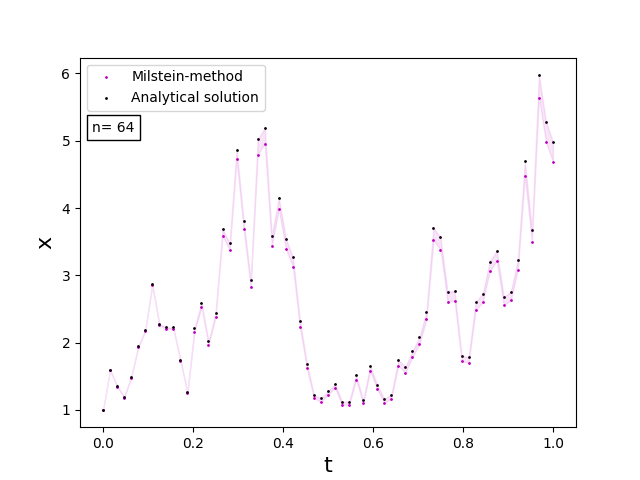
\includegraphics[scale=0.4]{Content/Graphics/Appendix/4gbm2}
   \end{subfigure}
   \begin{subfigure}{0.49\linewidth} \centering
     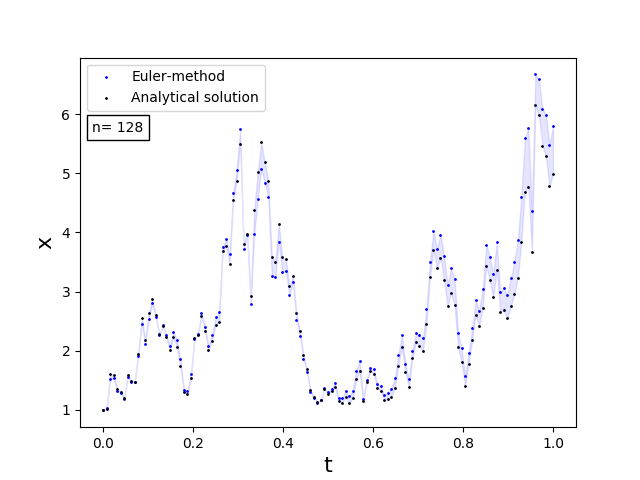
\includegraphics[scale=0.4]{Content/Graphics/Appendix/5gbm2}
   \end{subfigure}
   \begin{subfigure}{0.49\linewidth} \centering
     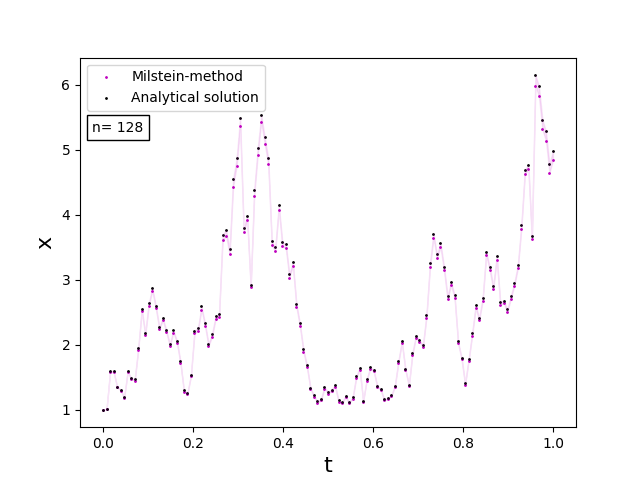
\includegraphics[scale=0.4]{Content/Graphics/Appendix/6gbm2}
   \end{subfigure}
\caption{Approximation (colored dots) of the sample path of the geometric Brownian motion and the true sample path (black dots) for n = 32, 64, 128 using Euler and Milstein.}
\end{figure}


\begin{figure}[!h]
\centering
   \begin{subfigure}{0.49\linewidth} \centering
     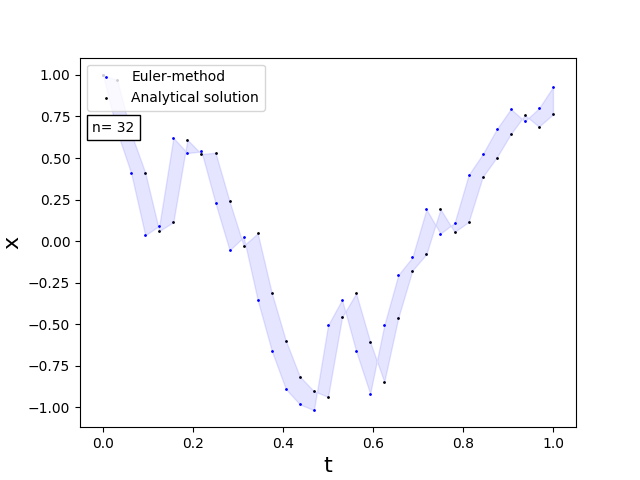
\includegraphics[scale=0.4]{Content/Graphics/Appendix/1ou}
   \end{subfigure}
   \begin{subfigure}{0.49\linewidth} \centering
     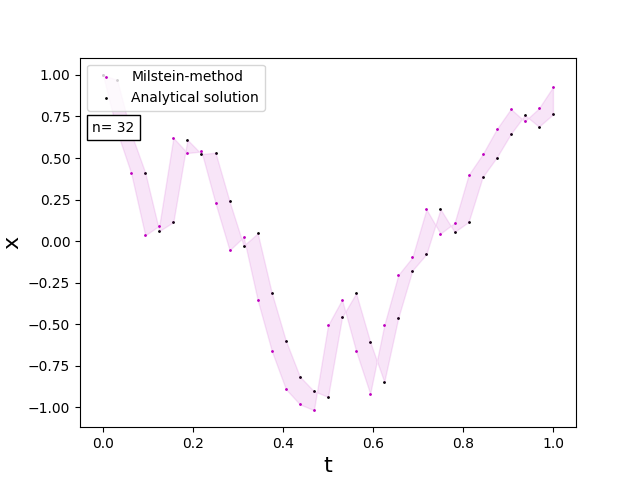
\includegraphics[scale=0.4]{Content/Graphics/Appendix/2ou}
   \end{subfigure}
   \begin{subfigure}{0.49\linewidth} \centering
     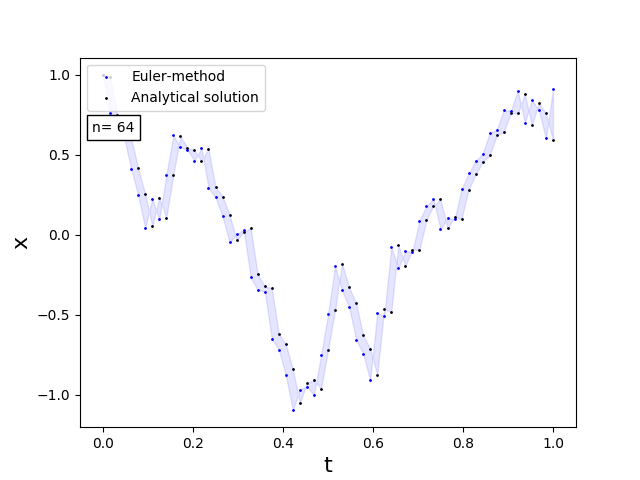
\includegraphics[scale=0.4]{Content/Graphics/Appendix/3ou}
   \end{subfigure}
   \begin{subfigure}{0.49\linewidth} \centering
     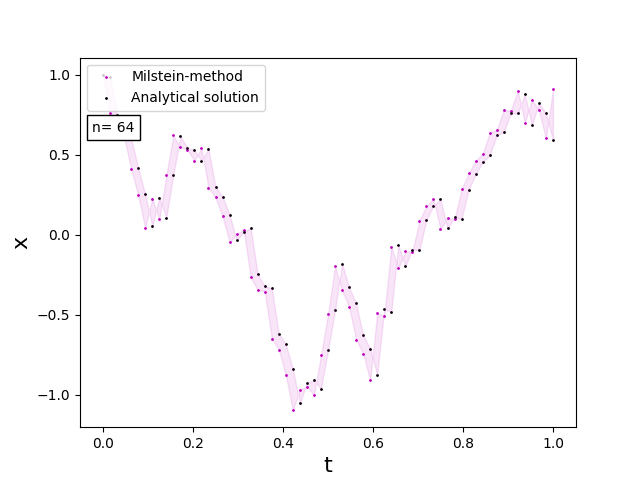
\includegraphics[scale=0.4]{Content/Graphics/Appendix/4ou}
   \end{subfigure}
   \begin{subfigure}{0.49\linewidth} \centering
     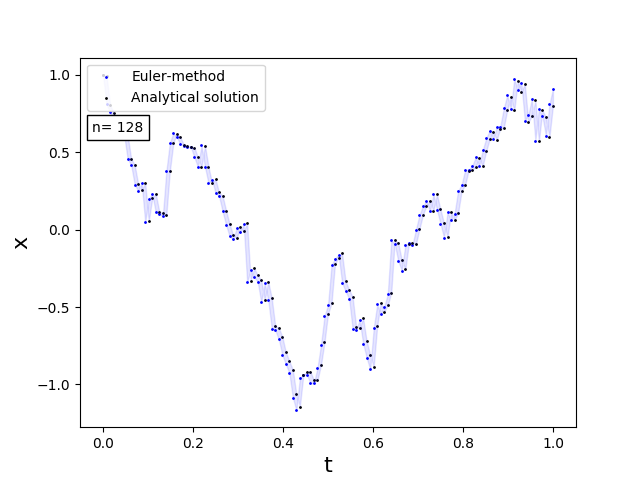
\includegraphics[scale=0.4]{Content/Graphics/Appendix/5ou}
   \end{subfigure}
   \begin{subfigure}{0.49\linewidth} \centering
     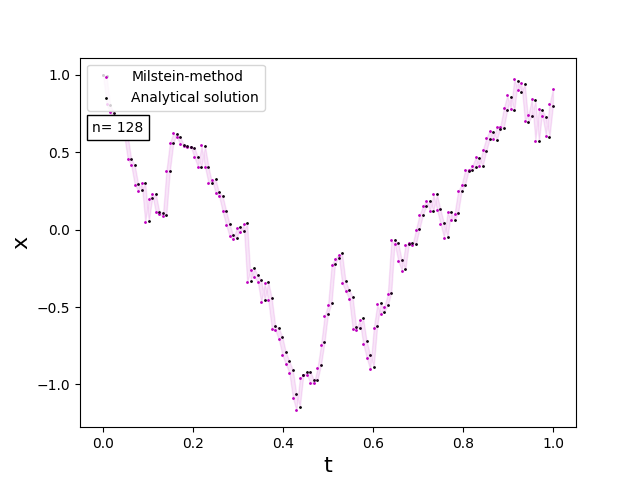
\includegraphics[scale=0.4]{Content/Graphics/Appendix/6ou}
   \end{subfigure}
\caption{Approximation (colored dots) of the sample path of the Ornstein-Uhlenbeck process and the true sample path (black dots) for n = 32, 64, 128 using Euler and Milstein.}
\end{figure}


\begin{figure}[!h]
\centering
   \begin{subfigure}{0.49\linewidth} \centering
     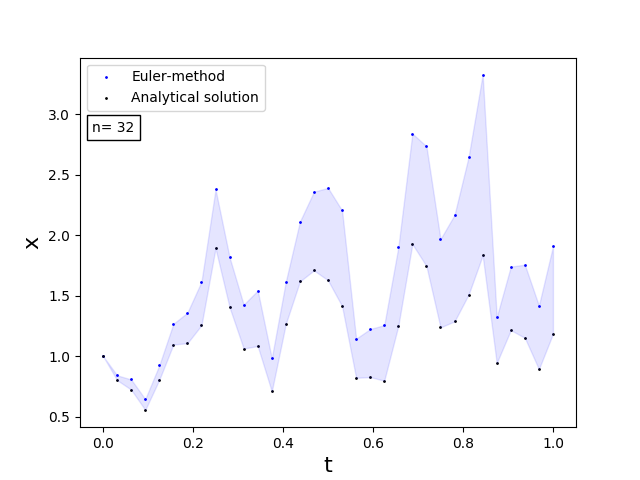
\includegraphics[scale=0.4]{Content/Graphics/Appendix/1gbm3}
   \end{subfigure}
   \begin{subfigure}{0.49\linewidth} \centering
     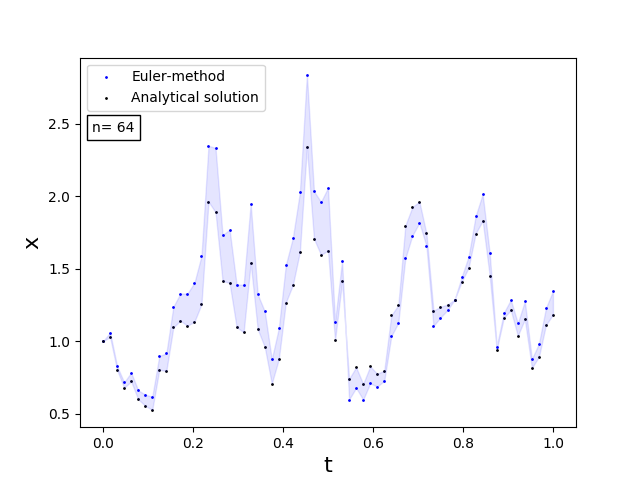
\includegraphics[scale=0.4]{Content/Graphics/Appendix/4gbm3}
   \end{subfigure}
   \begin{subfigure}{0.49\linewidth} \centering
     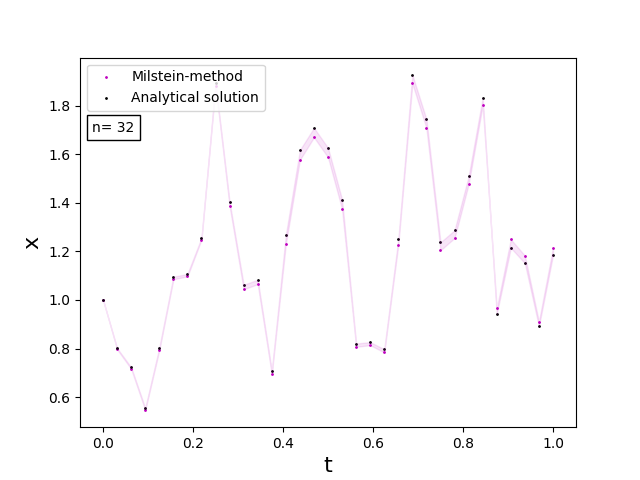
\includegraphics[scale=0.4]{Content/Graphics/Appendix/2gbm3}
   \end{subfigure}
   \begin{subfigure}{0.49\linewidth} \centering
     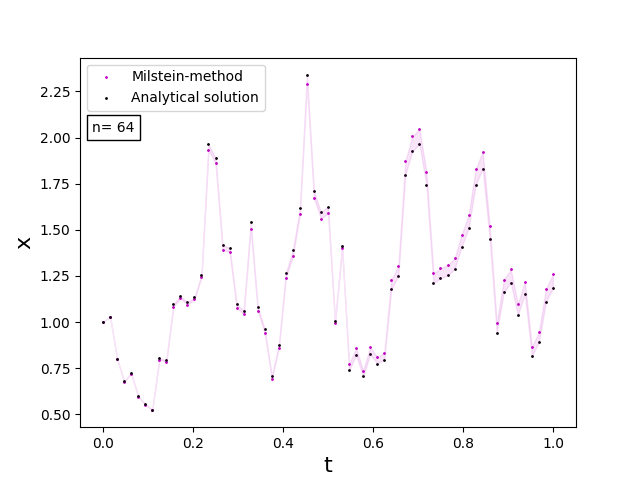
\includegraphics[scale=0.4]{Content/Graphics/Appendix/5gbm3}
   \end{subfigure}
   \begin{subfigure}{0.49\linewidth} \centering
     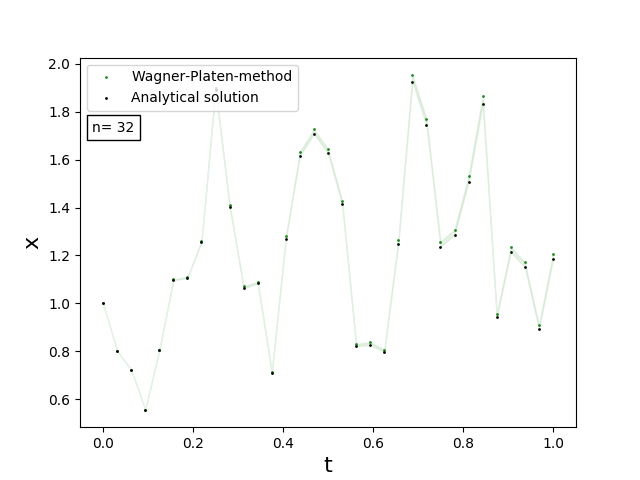
\includegraphics[scale=0.4]{Content/Graphics/Appendix/3gbm3}
   \end{subfigure}
   \begin{subfigure}{0.49\linewidth} \centering
     \includegraphics[scale=0.4]{Content/Graphics/Appendix/6gbm3}
   \end{subfigure}
\caption{Approximation (colored dots) of the sample path of the Ornstein-Uhlenbeck process and the true sample path (black dots) for n = 32, 64 using Euler, Milstein and Wagner-Platen.}
\end{figure}


\begin{figure}[!h]
     \includegraphics[scale=0.7]{Content/Graphics/Appendix/Error_analysis_gbm}
	\caption{Monte-Carlo estimates of the approximation error and the step amount n (logarithmized) for the geometric Brownian motion using Euler, Milstein, Wagner-Platen (20'000 simulations).}
\end{figure}
\begin{figure}[!h]
     \includegraphics[scale=0.7]{Content/Graphics/Appendix/Conv_order_gbm}
\caption{Log-log plot of the approximation error and the step amount n for the geometric Brownian motion using Euler, Milstein, Wagner-Platen (20'000 simulations).} 
\end{figure}


\backmatter

\nocite{*}
\bibliographystyle{plain}
\bibliography{Content/References}


\end{document}
